% ---------------------------------------------------------------------------------------------------------------
% TEMPLATE PARA TRABALHO DE CONCLUSÃO DE CURSO
% Universidade Tecnológica Federal do Paraná - UTFPR
% Customização da classe abnTeX2 (http://www.abntex.net.br/) para as normas da UTFPR
%
% Autores: Diego Marczal
% 	       Michael Vornes <https://github.com/mvornes>
% Adaptação (DACOM-CP): Silvio Ricardo Rodrigues Sanches
%
%----------------------------------------------------------------------------------------------------------------
% Codificação: UTF-8
% LaTeX:  abnTeX2          
% ---------------------------------------------------------------------------------------------------------------


% CARREGA CLASSE PERSONALIZADA DA UTFPR--------------------------------------------------------------------------
\documentclass[%twoside,                   % Impressão em frente e verso
    	        oneside,                   % Impressão apenas frente
]{configuracoes/utfpr-abntex2}

% INCLUI ARQUIVOS DE CONFIGURAÇÕES-------------------------------------------------------------------------------
% REFERÊNCIAS------------------------------------------------------------------
\usepackage[%
    alf,
    abnt-emphasize=bf,
    bibjustif,
    recuo=0cm,
    abnt-url-package=url,       % Utiliza o pacote url
    abnt-refinfo=yes,           % Utiliza o estilo bibliográfico abnt-refinfo
    abnt-etal-cite=3,
    abnt-etal-list=3,
    abnt-thesis-year=final
]{abntex2cite}                  % Configura as citações bibliográficas conforme a norma ABNT

% PACOTES----------------------------------------------------------------------
\usepackage[utf8]{inputenc}                                 % Codificação do documento
\usepackage[T1]{fontenc}                                    % Seleção de código de fonte
\usepackage{booktabs}                                       % Réguas horizontais em tabelas
\usepackage{color, colortbl}                                % Controle das cores
\usepackage{float}                                          % Necessário para tabelas/figuras em ambiente multi-colunas
\usepackage{graphicx}                                       % Inclusão de gráficos e figuras
\usepackage{icomma}                                         % Uso de vírgulas em expressões matemáticas
\usepackage{indentfirst}                                    % Indenta o primeiro parágrafo de cada seção
\usepackage{microtype}                                      % Melhora a justificação do documento
\usepackage{multirow, array}                                % Permite tabelas com múltiplas linhas e colunas
\usepackage{subeqnarray}                                    % Permite subnumeração de equações
\usepackage{lastpage}                                       % Para encontrar última página do documento
\usepackage{verbatim}                                       % Permite apresentar texto tal como escrito no documento, ainda que sejam comandos Latex
\usepackage{amsfonts, amssymb, amsmath}                     % Fontes e símbolos matemáticos
\usepackage[algoruled, portuguese]{algorithm2e}             % Permite escrever algoritmos em português
%\usepackage[scaled]{helvet}                                % Usa a fonte Helvetica
\usepackage{times}                                          % Usa a fonte Times
%\usepackage{palatino}                                      % Usa a fonte Palatino
%\usepackage{lmodern}                                       % Usa a fonte Latin Modern
\usepackage[bottom]{footmisc}                               % Mantém as notas de rodapé sempre na mesma posição
\usepackage{ae, aecompl}                                    % Fontes de alta qualidade
\usepackage{latexsym}                                       % Símbolos matemáticos
\usepackage{lscape}                                         % Permite páginas em modo "paisagem"
%\usepackage{picinpar}                                      % Dispor imagens em parágrafos
%\usepackage{scalefnt}                                      % Permite redimensionar tamanho da fonte
%\usepackage{subfig}                                        % Posicionamento de figuras
%\usepackage{upgreek}                                       % Fonte letras gregas

% Redefine a fonte para uma fonte similar a Arial (fonte Helvetica)
\renewcommand*\familydefault{\sfdefault}

% CONFIGURAÇÕES DE APARÊNCIA DO PDF FINAL--------------------------------------
\makeatletter
\hypersetup{%
    portuguese,
    colorlinks=true,   % true: "links" coloridos; false: "links" em caixas de texto
    linkcolor=blue,    % Define cor dos "links" internos
    citecolor=blue,    % Define cor dos "links" para as referências bibliográficas
    filecolor=blue,    % Define cor dos "links" para arquivos
    urlcolor=blue,     % Define a cor dos "hiperlinks"
    breaklinks=true,
    pdftitle={\@title},
    pdfauthor={\@author},
    pdfkeywords={abnt, latex, abntex, abntex2}
}
\makeatother

% ALTERA O ASPECTO DA COR AZUL--------------------------------------------------
\definecolor{blue}{RGB}{41,5,195}

% REDEFINIÇÃO DE LABELS---------------------------------------------------------
\renewcommand{\algorithmautorefname}{Algoritmo}
\def\equationautorefname~#1\null{Equa\c c\~ao~(#1)\null}

% CRIA ÍNDICE REMISSIVO---------------------------------------------------------
\makeindex

% HIFENIZAÇÃO DE PALAVRAS QUE NÃO ESTÃO NO DICIONÁRIO---------------------------
\hyphenation{%
    qua-dros-cha-ve
    Kat-sa-gge-los
}


\graphicspath{{./dados/}}

% INCLUI ARQUIVOS DO TRABALHO DE CONCLUSÃO DE CURSO (PRÉ-TEXTUAIS, TEXTUAIS, PÓS-TEXTUAIS)-----------------------

% INSERE CAPA E FOLHA DE ROSTO
% CAPA---------------------------------------------------------------------------------------------------

% ORIENTAÇÕES GERAIS-------------------------------------------------------------------------------------
% Caso algum dos campos não se aplique ao seu trabalho, como por exemplo,
% se não houve coorientador, apenas deixe vazio.
% Exemplos: 
% \coorientador{}
% \departamento{}

% DADOS DO TRABALHO--------------------------------------------------------------------------------------
\titulo{Título do Trabalho: Subtítulo do Trabalho}
\titleabstract{Title in English}
\autor{Nome Completo do Autor}
\autorcitacao{SOBRENOME, Nome} % Sobrenome em maiúsculo
\local{Cornélio Procópio}
\data{2018}

% NATUREZA DO TRABALHO-----------------------------------------------------------------------------------
% Opções: 
% - Trabalho de Conclusão de Curso (se for Graduação)
% - Dissertação (se for Mestrado)
% - Tese (se for Doutorado)
% - Projeto de Qualificação (se for Mestrado ou Doutorado)
\projeto{Trabalho de Conclusão de Curso}

% TÍTULO ACADÊMICO---------------------------------------------------------------------------------------
% Opções:
% - Bacharel ou Tecnólogo (Se a natureza for Trabalho de Conclusão de Curso)
% - Mestre (Se a natureza for Dissertação)
% - Doutor (Se a natureza for Tese)
% - Mestre ou Doutor (Se a natureza for Projeto de Qualificação)
\tituloAcademico{...}

% ÁREA DE CONCENTRAÇÃO E LINHA DE PESQUISA---------------------------------------------------------------
% Se a natureza for Trabalho de Conclusão de Curso, deixe ambos os campos vazios
% Se for programa de Pós-graduação, indique a área de concentração e a linha de pesquisa
\areaconcentracao{}
\linhapesquisa{}

% DADOS DA INSTITUIÇÃO-----------------------------------------------------------------------------------
% Se a natureza for Trabalho de Conclusão de Curso, coloque o nome do curso de graduação em "programa"
% Formato para o logo da Instituição: \logoinstituicao{<escala>}{<caminho/nome do arquivo>}
\instituicao{Universidade Tecnológica Federal do Paraná}
\departamento{Departamento Acadêmico de Computação}
\programa{Curso de ...}
\logoinstituicao{0.2}{dados/figuras/logo-instituicao.png} 

% DADOS DOS ORIENTADORES---------------------------------------------------------------------------------
\orientador{Nome do orientador}
%\orientador[Orientadora:]{Nome da orientadora}
\instOrientador{Instituição do orientador}

\coorientador{Nome do coorientador}
%\coorientador[Coorientadora:]{Nome da coorientadora}
\instCoorientador{Instituição do coorientador}

% FOLHA DE ROSTO--------------------------------------------------------------------------------------------------------

% TRABALHO DE CONCLUSÃO DE CURSO
 \preambulo{{\imprimirprojeto} apresentado ao {\imprimirprograma} da {\imprimirinstituicao}, como requisito parcial para a obtenção do título de {\imprimirtituloAcademico}.}

% DISSERTAÇÃO DE MESTRADO
% \preambulo{{\imprimirprojeto} apresentada ao Programa de \mbox{Pós-graduação} da {\imprimirinstituicao}, como requisito parcial para obtenção do título de {\imprimirtituloAcademico}.}

% TESE DE DOUTORADO
% \preambulo{{\imprimirprojeto} apresentada ao Programa de \mbox{Pós-graduação} da {\imprimirinstituicao}, como requisito parcial para a obtenção do título de {\imprimirtituloAcademico}.}

% PROJETO DE QUALIFICAÇÃO DE MESTRADO OU DOUTORADO
%\preambulo{{\imprimirprojeto} apresentado ao Programa de \mbox{Pós-graduação} da {\imprimirinstituicao}, como requisito parcial para a obtenção do título de {\imprimirtituloAcademico}.}

% OBSERVAÇÕES-----------------------------------------------------------------------------------------------------------
% Altere este arquivo APENAS comentando as linhas que não se aplicam ao tipo de trabalho acadêmico desejado.


\begin{document}

\pretextual
\imprimircapa                                               	           % Comando para imprimir Capa
\imprimirfolhaderosto{}                                     		   % Comando para imprimir Folha de rosto
% INSERE ELEMENTOS PRÉ-TEXTUAIS
%% DEDICATÓRIA------------------------------------------------------------------

\renewcommand{\dedicatorianame}{DEDICATÓRIA}

\begin{dedicatoria}

Altere este texto inserindo a dedicatória do seu trabalho. 

\end{dedicatoria}
          			   % Dedicatória
%% AGRADECIMENTOS---------------------------------------------------------------

\begin{agradecimentos}[AGRADECIMENTOS]

Edite e coloque aqui os agradecimentos às pessoas e/ou instituições que contribuíram para a realização do trabalho.

É obrigatório o agradecimento às instituições de fomento à pesquisa que financiaram total ou parcialmente o trabalho, inclusive no que diz respeito à concessão de bolsas.

\end{agradecimentos}
        			   % Agradecimentos
%% EPÍGRAFE---------------------------------------------------------------------

\renewcommand{\epigraphname}{EPÍGRAFE}

\begin{epigrafe}

\textit{Eu denomino meu campo de Gestão do Conhecimento, mas você não pode gerenciar conhecimento. Ninguém pode. O que pode fazer - o que a empresa pode fazer - é gerenciar o ambiente que otimize o conhecimento. (PRUSAK, Laurence, 1997).}

\end{epigrafe}

% OBSERVAÇÕES------------------------------------------------------------------
% Altere o texto para inserir a epígrafe do seu trabalho
              			   % Epígrafe
% RESUMO--------------------------------------------------------------------------------

\begin{resumo}[RESUMO]
\begin{SingleSpacing}

% Não altere esta seção do texto--------------------------------------------------------
\imprimirautorcitacao. \imprimirtitulo. \imprimirdata. \pageref {LastPage} f. \imprimirprojeto\ – \imprimirprograma, \imprimirinstituicao. \imprimirlocal, \imprimirdata.\\
%---------------------------------------------------------------------------------------

O Resumo é um elemento obrigatório em tese, dissertação, monografia e TCC, constituído de uma seqüência de frases concisas e objetivas, fornecendo uma visão rápida e clara do conteúdo do estudo. O texto deverá conter no máximo 500 palavras e ser antecedido
pela referência do estudo. Também, não deve conter citações. O resumo deve ser redigido em parágrafo único, espaçamento simples e seguido das palavras representativas do conteúdo do estudo, isto é, palavras-chave, em número de três a cinco, separadas entre si por ponto e finalizadas também por ponto. Usar o verbo na terceira pessoa do singular, com linguagem impessoal, bem como fazer uso, preferencialmente, da voz ativa. Texto contendo um único parágrafo.\\

\textbf{Palavras-chave}: Palavra. Segunda Palavra. Outra palavra.

\end{SingleSpacing}
\end{resumo}

% OBSERVAÇÕES---------------------------------------------------------------------------
% Altere o texto inserindo o Resumo do seu trabalho.
% Escolha de 3 a 5 palavras ou termos que descrevam bem o seu trabalho 
             			   % Resumo em Português
% ABSTRACT--------------------------------------------------------------------------------

\begin{resumo}[ABSTRACT]
\begin{SingleSpacing}

% Não altere esta seção do texto--------------------------------------------------------
\imprimirautorcitacao. \imprimirtitleabstract. \imprimirdata. \pageref {LastPage} f. \imprimirprojeto\ – \imprimirprograma, \imprimirinstituicao. \imprimirlocal, \imprimirdata.\\
%---------------------------------------------------------------------------------------

Elemento obrigatório em tese, dissertação, monografia e TCC. É a versão do resumo em português para o idioma de divulgação internacional. Deve ser antecedido pela referência do estudo. Deve aparecer em folha distinta do resumo em língua portuguesa e seguido das palavras representativas do conteúdo do estudo, isto é, das palavras-chave. Sugere-se a elaboração do resumo (Abstract) e das palavras-chave (Keywords) em inglês; para resumos em outras línguas, que não o inglês, consultar o departamento / curso de origem.\\

\textbf{Keywords}: Word. Second Word. Another word.

\end{SingleSpacing}
\end{resumo}

% OBSERVAÇÕES---------------------------------------------------------------------------
% Altere o texto inserindo o Abstract do seu trabalho.
% Escolha de 3 a 5 palavras ou termos que descrevam bem o seu trabalho 
             		           % Resumo em Inglês
% Lista de Figuras----------------------------------------------------------------

\pdfbookmark[0]{\listfigurename}{lof}
\listoffigures*
\cleardoublepage

% OBSERVAÇÕES---------------------------------------------------------------------
% Este arquivo não precisa de ser alterado, pois a lista é gerada automaticamente.
   % Lista de Figuras
% LISTA DE QUADROS----------------------------------------------------------------

\renewcommand{\listofquadrosname}{LISTA DE QUADROS}

\pdfbookmark[0]{\listofquadrosname}{loq}
\listofquadros*
\cleardoublepage

% OBSERVAÇÕES---------------------------------------------------------------------
% Este arquivo não necessita de ser editado. A lista é gerada automaticamente.
   % Lista de Quadros
% LISTA DE TABELAS-------------------------------------------------------------

\pdfbookmark[0]{\listtablename}{lot}
\listoftables*
\cleardoublepage

% OBSERVAÇÕES-------------------------------------------------------------------
% Este arquivo não precisa ser alterado, pois a lista é gerada automaticamente.
         		   % Lista de Tabelas
% LISTA DE ABREVIATURAS E SIGLAS----------------------------------------------------------

\begin{siglas}
    \item[ABNT] Associação Brasileira de Normas Técnicas
    \item[DECOM] Departamento de Computação
\end{siglas}

% OBSERVAÇÕES-----------------------------------------------------------------------------
% Altere a lista acima para definir os acrônimos e siglas utilizados neste trabalho
          		   % Lista de Abreviaturas e Siglas
%% LISTA DE SÍMBOLOS------------------------------------------------------------

\begin{simbolos}
    \item[$ \Gamma $] Letra grega Gama
    \item[$ \lambda $] Comprimento de onda
    \item[$ \in $] Pertence
\end{simbolos}

% OBSERVAÇÕES-------------------------------------------------------------------
% Altere a lista acima para definir os símbolos utilizados no trabalho
        		   % Lista de Símbolos
%% LISTA DE ALGORITMOS----------------------------------------------------------

\newcommand{\algoritmoname}{Algoritmo}
\renewcommand{\listalgorithmcfname}{LISTA DE ALGORITMOS}

\floatname{algocf}{\algoritmoname}
\newlistof{listofalgoritmos}{loa}{\listalgoritmoname}
\newlistentry{algocf}{loa}{0}

\counterwithout{algocf}{chapter}
\renewcommand{\cftalgocfname}{\algoritmoname\space}
\renewcommand*{\cftalgocfaftersnum}{\hfill--\hfill}

\pdfbookmark[0]{\listalgorithmcfname}{loa}
\listofalgorithms
\cleardoublepage

% OBSERVAÇÕES------------------------------------------------------------------
% Este arquivo não precisa ser alterado, pois a lista é gerada automaticamente.
   % Lista de Algoritmos
% SUMÁRIO----------------------------------------------------------------------

\renewcommand{\contentsname}{SUMÁRIO}

\pdfbookmark[0]{\contentsname}{toc}
\tableofcontents*
\cleardoublepage

% OBSERVAÇÕES-------------------------------------------------------------------
% Este arquivo não precisa ser alterado, pois o sumário é gerado automaticamente.
               			   % Sumário

\textual
% INSERE ELEMENTOS TEXTUAIS
% INTRODUÇÃO-------------------------------------------------------------------

\chapter{INTRODUÇÃO}
\label{chap:introducao}

Edite e coloque aqui o seu texto de introdução.

A Introdução é a parte inicial do texto, na qual devem constar o tema e a delimitação do assunto tratado, objetivos da pesquisa e outros elementos necessários para situar o tema do trabalho, tais como: justificativa, procedimentos metodológicos (classificação inicial), embasamento teórico (principais bases sintetizadas) e estrutura do trabalho, tratados de forma sucinta. Recursos utilizados e cronograma são incluídos quando necessário. Salienta-se que os procedimentos metodológicos e o embasamento teórico são tratados, posteriormente, em capítulos próprios e com a profundidade necessária ao trabalho de pesquisa.

\section{LEIA ESTA SEÇÃO ANTES DE COMEÇAR}
\label{sec:antesleiame}

Este documento é um \emph{template} \LaTeX{} que foi concebido, primariamente, para ser utilizado na elaboração de Trabalho de Conclusão de Curs em conformidade com as normas da Universidade Tecnológica Federal do Paraná.

Para a produção deste \emph{template} foi necessário adaptar o arquivo {\ttfamily abntex2.cls}. Assim, foi produzido o arquivo {\ttfamily utfpr-abntex2.cls} que define o \verb|documentclass| específico para a UTFPR.

Antes de começar a escrever o seu trabalho acadêmico utilizando este \emph{template}, é importante saber que há dois arquivos que você precisará editar para que a capa e a folha de rosto de seu trabalho sejam geradas automaticamente.
São eles os arquivos {\ttfamily capa.tex} e {\ttfamily folha-rosto.tex}, ambos no diretório  {\ttfamily /elementos-pre-textuais}.
No arquivo {\ttfamily capa.tex} deverá ser informado nome do autor, título do trabalho, natureza do trabalho, nome do orientador e outras informações necessárias.
No arquivo {\ttfamily folha-rosto.tex}, que contém o texto padrão estabelecendo que este documento é um requisito parcial para a obtenção do título pretendido, será necessário apenas comentar as linhas que não se aplicam ao tipo de trabalho acadêmico.

A compilação para gerar um arquivo no formato pdf, incluindo corretamente as referências bibliográficas, deve ser realizada utilizando o comando \verb|makefile|, disponível na mesma pasta onde está o arquivo principal \verb|utfpr-tcc.tex|. Caso seja alterado o nome do arquivo \verb|utfpr-tcc.tex|, deverá ser alterado no arquivo \verb|makefile| também.

\section{ORGANIZAÇÃO DO TRABALHO}
\label{sec:organizacaoTrabalho}

Normalmente ao final da introdução é apresentada, em um ou dois parágrafos curtos, a organização do restante do trabalho acadêmico.
Deve-se dizer o quê será apresentado em cada um dos demais capítulos.
                		           % Introdução
% FUNDAMENTACAO ------------------------------------------------------------------

\chapter{FUNDAMENTAÇÃO TEÓRICA}
\label{chap:fundamentacao}

\section{EMATER}
\label{subsec:emater}

O Instituto Paranaense de Assistência Técnica e Extensão Rural (EMATER) é uma autarquia vinculada à Secretaria de Estado da Agricultura e Abastecimento, que tem o papel de executar o serviço oficial de extensão rural do Estado \cite{ematerAE}.
A extensão rural tem como meta o progresso rural sustentável, por meio de assistência técnica focada na melhoria de renda dos agricultores em seus empreendimentos, qualidade de vida nas famílias no ambiente rural, avanço na competitividade e preservação dos recursos naturais e o meio ambiente.

A extensão rural oficial é disponibilizada em praticamente todo o estado. São 395 unidades que estendem aos agricultores de todos os municípios. Os beneficiários do processo de orientação são privilegiados os projetos que atendam as necessidades locais e regionais.

\section{PROGRAMA DE APOIO AO MANEJO E FERTILIDADE DO SOLO}
\label{subsec:pamfs}

O Programa de Apoio ao Manejo e Fertilidade do Solo, conhecido como Programa de Calcário, proporciona o uso de corretivos de solo aos agricultores familiares menos favorecidos, em busca do aumento de produtividade. O projeto ainda auxilia o pequeno agricultor na organização do processo de correção do solo, desde a identificação da necessidade de correção até a aplicação, incluindo o transporte e armazenagem \cite{ematerPAMFS}.

Entre os anos de 2013 e 2014, o programa beneficiou cerca de 35 mil produtores, aplicando aproximadamente 350 milhões de quilos de corretivos no solo, investindo entorno de 33,5 milhões de reais.

O Instituto Emater é responsável pela organização e aplicação do programa, divulgando, auxiliando na seleção dos favorecidos e definindo juntamente com os parceiros os planos de execução.

Além disso, o Instituto Emater também é responsável pela elaboração de projetos técnicos, pela orientação aos agricultores na coleta de amostras de solo e na recomendação do uso de corretivos agrícolas.

\section{CORREÇÃO E EQUILÍBRIO DO SOLO}
\label{subsec:correcaodosolo}

A terra é o elemento central da agricultura e precisa de um bom manejo para que haja uma boa safra. Mesmo que seja feita uma boa adubação, algumas plantas, como a soja e o milho, não se desenvolvem bem em um pH ácido \cite{de2003sugestao}, pois a disponibilidade de nutrientes está diretamente relacionada à acidez do solo. Por isso, a correção do solo pode ser determinante para uma colheita farta ou mediana, contribuindo para o aumento da renda e, consequentemente, da qualidade de vida do produtor rural.

Diversos fatores contribuem para o desempenho do terreno como a compactação do solo e a pluviosidade, mas a acidez é o principal deles. Devido à fatores geológicos, o Brasil tende a possuir uma grande concentração de íons de hidrogênio e alumínio \cite{bookfa2215c6}. Dessa forma, nutrientes essenciais como nitrogênio, fósforo e potássio têm sua disponibilidade comprometida, afetando o crescimento do vegetal.

O alumínio e manganês, quando disponibilizados em excesso, são tóxicos para a plantação \cite{malavolta1980effects}. Ao contrário dos nutrientes supracitados, esses aumentam quando o pH diminui. A presença desses elementos prejudicam o desenvolvimento do sistema radicular, muitas vezes causando o tombamento da planta, prejudicando a absorção de nutrientes e a produtividade da cultura.

Para aumentar o pH, deve-se realizar a calagem , que é a aplicação de calcário no terreno \cite{rossetto}. A qualidade e rapidez de incorporação e a dose recomendada do calcário está diretamente relacionada ao Poder Real de Neutralização Total (PRNT) do corretivo.

\section{PLANILHA DE CORREÇÃO DE SOLOS}
\label{subsec:planilha}

Atualmente a Emater utiliza uma planilha eletrônica desenvolvida para o Microsoft Excel por Pedro Cecere Filho e Fabianderson J. B. de Souza e contou com o apoio de Nelson Hargerm, Celso D. Seratto e Adilson O. Junior, para a realização dos cálculos de correção e equilíbrio do solo.

O objetivo dessa planilha é gerar um relatório de recomendações para a correção do solo de um determinado talhão com base no laudo técnico do solo, na cultura desejada, na produtividade desejada. Além disso a planilha também fornece a quantidade e o valor aproximado de cada corretivo agrícola que o produtor deverá adquirir para suprir as necessidades da planta. 

A planilha é composta por 5 pastas de trabalho que serão enumeradas e descritas nas subseções abaixo.

\subsection{Pasta de Trabalho: Ajuda}
\label{subsec:pastaajuda}

Nessa pasta estão descritas algumas instruções para o correto uso da planilha, bem como os créditos aos participantes no desenvolvimento, o telefone de contato do técnico responsável para esclarecimento de dúvidas e a data da última atualização, conforme é exibido na \autoref{fig:pastaajuda}.

\begin{figure}[H]
    \centering
    \caption{Pasta de Trabalho: Ajuda}
    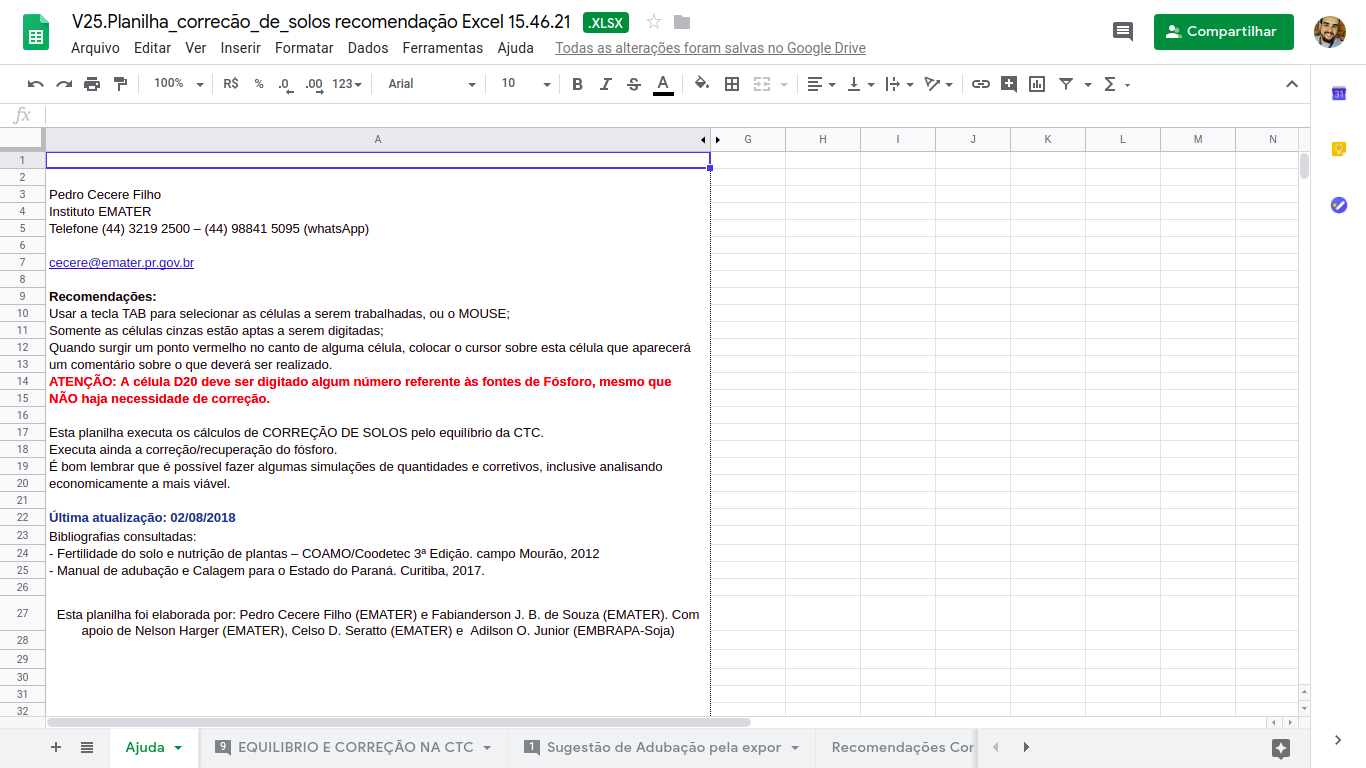
\includegraphics[width=13cm]{dados/figuras/planilha/tab-ajuda.png}
    \label{fig:pastaajuda}
    \fonte{Planilha de Correção do Solo}
\end{figure}

\subsection{Pasta de Trabalho: Equilíbrio e Correção na CTC}
\label{subsec:pastaequilibriocorrecaoctc}

Esta é a pasta de trabalho na qual o técnico informa os dados acerca do local a ser corrigido. Para facilitar o entendimento, o formulário será dividido em 5 seções que estão descritas nas próximas subseções. Deve-se considerar que os campos com o fundo em cinza são entradas do usuário.

O objetivo dessa pasta é fornecer uma visão geral dos três momentos da área analisada: como ela está atualmente, como ela deverá estar após as correções e como seria no caso ideal. O valor ideal depende da cultura considerada para o talhão. A planilha apresentada só considera as possibilidades de cultivo de soja e milho nas áreas corrigidas.

É importante salientar que existem diferentes métodos de avaliação para a calagem do solo. Porém, a planilha aborda apenas o método de saturação por bases. Este é o método é praticado apenas nas regiões de SP e PR \cite{rossetto}.

\subsubsection{Identificação da Propriedade}
\label{subsubsec:identificacao}
Esta seção é responsável pela entrada de dados referentes ao local de coleta da amostra de terra, denominado talhão, enviada para a análise em laboratório. Para identificação do talhão a planilha solicita ao usuário as seguintes entradas: do nome do proprietário, a data do cálculo, o município e lote onde esta está situada, a área total em hectares, a identificação do talhão, a área do talhão em hectares e a matrícula do lote além do nome do técnico da Emater responsável por essa região e o tipo de plantio aplicado, que pode ser o convencional ou direto.

\begin{figure}[H]
    \centering
    \caption{Identificação do Talhão}
    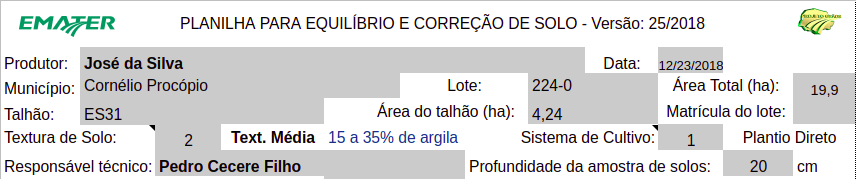
\includegraphics[width=13cm]{dados/figuras/planilha/corr_info_propriedade.png}
    \label{fig:identificacaotalhao}
    \fonte{Planilha de Correção do Solo}
\end{figure}

Outros dados relevantes para o cálculo da correção do solo como profundidade da amostra em centímetros e textura do solo, que pode ser argilosa ou textura média dependendo da proporção de argila, também são colhidos nessa seção.

\subsubsection{Resultado da Análise Química do Solo}
\label{subsubsec:analisequimica}

O laudo técnico do solo é emitido por um laboratório de análise do solo e possui um número de identificação. Ele apresenta as características físicas e químicas do solo. Dentre as características físicas, a textura do solo é indispensável para o cálculo da correção. Outras informações como profundidade da amostra coletada e o sistema de cultivo também são importantes.

A planilha considera apenas duas variações de textura do solo: o argiloso e o de textura média. O solo argiloso é aquele que possui argila em pelo menos 35\% de sua composição, enquanto o de textura média varia entre 15\% e 35\%.

Os teores de nutrientes do solo também são provenientes do laudo técnico, que pode ser observado no \autoref{chap:laudodosolo}. Os nutrientes considerados na planilha são o fósforo (P), o potássio (K), o Cálcio (Ca), o Magnésio (Mg), o Enxofre (S), o Alumínio (Al) e a acidez potencial (soma do Hidrogênio e o Alumínio). Os valores de P são informados em \(mg/dm^3\), enquanto o K, Ca, Mg, S, H e Al são fornecidos em \(cmol/dm^3\).

\begin{figure}[H]
    \centering
    \caption{Laudo Técnico do Solo}
    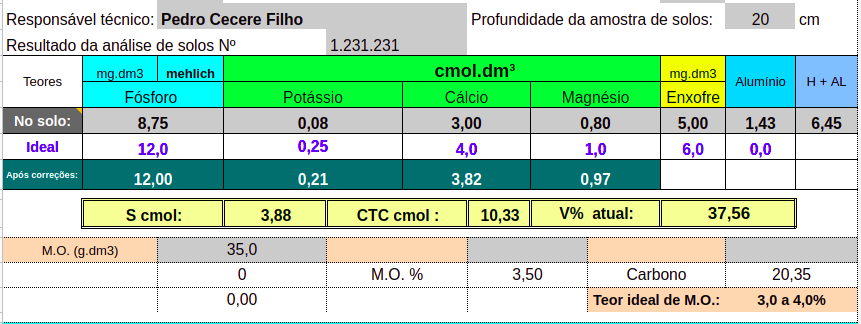
\includegraphics[width=13cm]{./dados/figuras/planilha/corr_analise_quimica.png}
    \label{fig:analisequimicatabela}
    \fonte{Planilha de Correção do Solo}
\end{figure}

A planilha calcula e exibe dinamicamente os valores ideais dos nutrientes de acordo com a textura do solo e também qual será o teor de cada substância após a aplicação das correções.

Ainda na seção de análise do solo, o técnico informa o teor de matéria orgânica presente no solo. Como a unidade de medida depende do laboratório que emitiu o laudo, esse valor pode ser informado em \(g/dm^3\), percentual (\%) ou em carbono.

\subsubsection{Correção/Recuperação do Fósforo}
\label{subsubsec:corrrecfosforo}

Na seção de correção/recuperação do fósforo, o usuário deve fornecer informações para o cálculo de equilíbrio referente ao fósforo. O técnico deve informar qual é o teor desejado de fósforo em \(mg/dm^3\), qual será o corretivo será aplicado, a eficiência do fósforo do corretivo em percentual e o valor em R\$/ton da fonte de fósforo.

\begin{figure}[H]
    \centering
    \caption{Correção/Recuperação do Fósforo}
    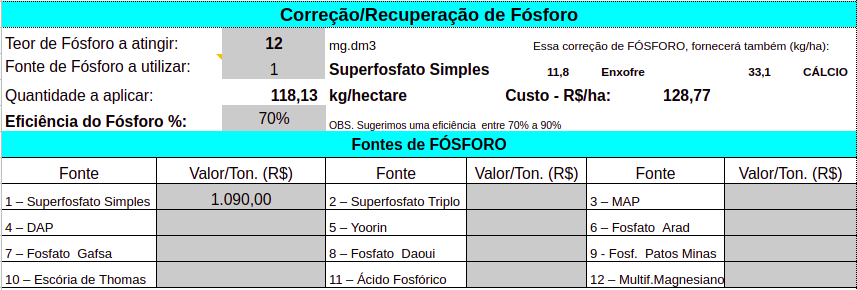
\includegraphics[width=13cm]{./dados/figuras/planilha/corr_rec_fosforo.png}
    \label{fig:correcaorecfosforo}
    \fonte{Planilha correção de solos}
\end{figure}

Após o preenchimento dos campos, o sistema consegue calcular ativamente a quantidade a ser aplicada e o custo em R\$/ha do fertilizante, além da quantidade em quilos de outros nutrientes que esta aplicação incrementará ao solo.

\subsubsection{Correção/Recuperação do Potássio}
\label{subsubsec:corrrecpotassio}

Nesta seção, a planilha exibe ao técnico o percentual da participação do potássio atualmente na CTC, solicita o percentual desejado, exibe o percentual ideal, exibe o percentual que esperado após as correções, além de solicitar a fonte de potássio e o custo em R\$/ton desse corretivo.

\begin{figure}[H]
    \centering
    \caption{Correção/Recuperação do potássio}
    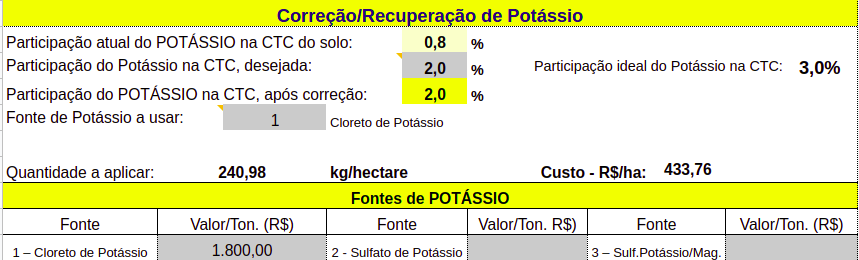
\includegraphics[width=13cm]{./dados/figuras/planilha/corr_rec_potassio.png}
    \label{fig:correcaorecpotassio}
    \fonte{Planilha correção de solos}
\end{figure}

Após o preenchimento dos campos em cinza, o sistema calcula e exibe dinamicamente a quantidade a ser aplicada e o custo em R\$/ha do fertilizante, além da quantidade em quilos de outros nutrientes que este corretivo fornecerá.

\subsubsection{Correção/Recuperação do Cálcio e Magnésio}
\label{subsubsec:corrreccalciomagnesio}

Nessa última seção de correção, a planilha recebe as entradas referentes à correção/recuperação do cálcio e magnésio. Nessa parte a planilha exibe o percentual de cálcio e magnésio presentes atualmente e o percentual ideal desses nutrientes na CTC de acordo com a textura de solo selecionada. Espera-se como entrada o percentual de cálcio desejado na CTC, a fonte de cálcio que será utilizada na correção e o custo em R\$/ton, além do PRNT e o teor de CaO da fonte de corretivo.

\begin{figure}[H]
    \centering
    \caption{Correção/Recuperação do Cálcio e Magnésio}
    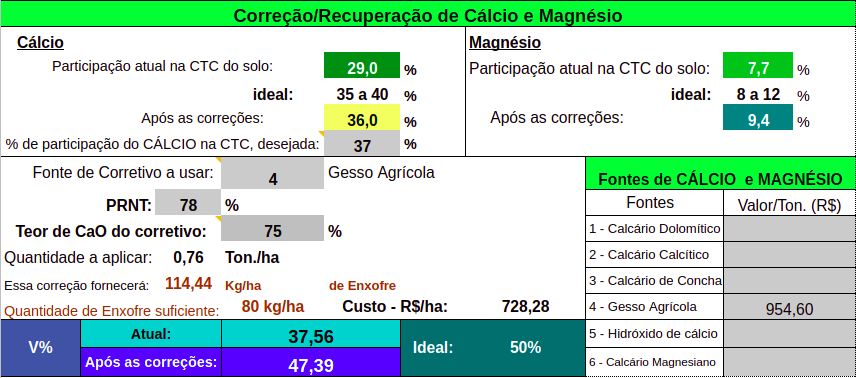
\includegraphics[width=13cm]{./dados/figuras/planilha/corr_rec_calcio_magnesio.png}
    \label{fig:correcaoreccalciomagnesio}
    \fonte{Planilha correção de solos}
\end{figure}

Com essas informações preenchidas, o sistema é capaz de calcular dinamicamente a quantidade da fonte de corretivo necessária para a correção em ton/ha, o custo em R\$/ha e a quantidade de outros nutrientes como o enxofre e que serão fornecidos à mistura. Além disso, também será possível informar o teor de Magnésio no solo após as correções.

O cálculo da necessidade de calagem se dá pela seguinte fórmula:

\[ NC
  = \dfrac{(V2 - V1) * CTC}{10 * PRNT}
\]

Sendo que:
\begin{itemize}
    \item NC: Necessidade de calagem
    \item V2: Saturação de bases desejada
    \item V1: Saturação de bases encontrada no solo
    \item CTC é a capacidade de troca de cátions, ou \(Ca + Mg + K + Na + (H + Al)\)
    \item PRNT: Poder Relativo de Neutralização Total
\end{itemize}

\subsubsection{Saturação por Bases}
\label{subsubsec:resultadosaturacao}

Nas últimas linhas da planilha desta pasta de trabalho são calculados os valores da saturação por bases (V\%) obtidos por meio dos cálculos com as informações fornecidas pelo usuário, como pode ser observado na \autoref{fig:saturacaoporbase}.

\begin{figure}[H]
    \centering
    \caption{Saturação de Base}
    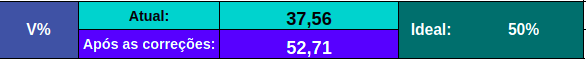
\includegraphics[width=13cm]{./dados/figuras/planilha/corr_saturacao.png}
    \label{fig:saturacaoporbase}
    \fonte{Planilha correção de solos}
\end{figure}

O valor de V\% representa o equilíbrio das bases na CTC. No caso do milho e da soja, para o melhor desenvolvimento desses vegetais, recomenda-se a saturação em 50\%.

\subsection{Pasta de Trabalho: Sugestão de adubação pela exportação}
\label{subsec:sugestaoadubacao}

Essa pasta de trabalho tem como objetivo gerar um plano de correção do solo baseado nas informações processadas na \autoref{subsec:pastaequilibriocorrecaoctc}. O usuário deve informar qual é a cultura que será destinada aquele talhão e a produtividade esperada em sacas/alqueire, além do percentual de eficiência fósforo do corretivo.

\subsection{Pasta de Trabalho: Memória de Cálculo}
\label{subsec:memoriadecalculo}

Essa pasta de trabalho armazena as fórmulas para a correção do fósforo, potássio, cálcio e magnésio e está dividida em 3 seções.

\subsection{Pasta de Trabalho: Recomendações Correção e Adubação}
\label{subsec:recomendacoes}

Essa pasta de trabalho é responsável pela geração do documento final de orientação de correção. Nela o técnico descreve como deverá ser corrigido cada um dos indicadores, indicando a quantidade e o valor em R\$/tonelada de cada corretivo.
No rodapé são dispostos dois campos para que o proprietário e o técnico façam a assinatura da recomendação.

\section{TRABALHOS RELACIONADOS}
\label{sec:trabalhosrelacionados}

\subsection{Nutrient Management Support System}
\label{sub:numass}

%https://ainfo.cnptia.embrapa.br/digital/bitstream/item/91181/1/FD345.pdf

\subsection{Agrowin}
\label{sub:agrowin}

%http://www.adubecerto.com.br/

\subsection{Comparativo}
\label{sub:comparativo}
                   % Fundamentação
% TÉCNICAS E FERRAMENTAS ------------------------------------------------------------------

\chapter{PROPOSTA}
\label{chap:proposta}

Neste capítulo serão expostas as tecnologias e ferramentas que serão utilizadas no desenvolvimento do aplicativo, bem como a metodologia que será seguida para o gerenciamento de tarefas.

\section{TECNOLOGIAS}
\label{sec:tecnologias}

A presente proposta diz respeito ao desenvolvimento de um sistema \textit{web}. Um sistema \textit{web} consiste em um programa de computador instalado em um servidor HTTP, que disponibiliza páginas \textit{web} para os clientes HTTP como \textit{web browsers}.

As tecnologias necessárias para o desenvolvimento da aplicação identificadas serão descritas abaixo.

\subsection{Unified Modeling Language}
\label{sub:uml}

A UML foi adotada como a linguagem de modelagem de sistema, pois com ela conseguimos facilmente representar comportamentos e necessidades do sistema em nível de software e \textit{hardware}. Os diagramas a serem modelados e suas respectivas funções são:

\begin{itemize}
    \item \textbf{Diagrama de Caso de Uso}, que fornecerá uma visão geral das funcionalidades do aplicativo.
    
    \item \textbf{Diagrama de Classe}, que possibilita o desenvolvedor entender a organização das classes e seus relacionamentos.
    
    \item \textbf{Diagrama de Implantação}, que proporciona uma visão de alto nível acerca das necessidade de hardware e software para a implantação da aplicação.
    
    \item \textbf{Diagrama Entidade-Relacionamento}, permite entender a organização dos dados nas tabelas, bem como os atributos, relacionamentos e restrições.
\end{itemize}

\subsection{MySQL}
\label{sub:rdb}

O MySQL será o SGBD para a persistência de dados. Ele foi escolhido devido à sua confiabilidade, consistência e normalização ante aos modelo não relacionais. É um sistema gratuito, amplamente utilizado em aplicações de todos os tamanhos. O uso desse SGBD utilizado pelo aplicativo da Uber \cite{klitzkeevan2016} e no portal openNASA \cite{howardalex2011}.

A modelagem do banco de dados foi feita utilizando a ferramenta MySQL Workbench e pode ser visualizado na \autoref{fig:diagramaer}. Já o dicionário de dados está disponível na \autoref{sec:titSecDiagERDicionario}.

\subsection{PHP}
\label{sub:php}

O Pre-hypertext Processor (PHP) é uma linguagem interpretada criada em 1995 por Rasmus Lerdorf. Amplamente utilizada no desenvolvimento de aplicações web, a linguagem evoluiu e passou a oferecer funcionalidades na linha de comando. Ela está presente no código fonte de grandes aplicações como Magento, WordPress, Drupal, Wikipédia e Facebook (até 2018) \cite{emmottfred2019}.

No presente projeto esta linguagem será utilizada no backend, por meio do Laravel Framework.

\subsection{Laravel \textit{Framework}}
\label{sub:laravel}

\citeonline{Sommerville10} afirma que, “os frameworks dão suporte ao reúso de projeto, bem como ao reúso de classes específicas de sistema, pois fornecem uma arquitetura de esqueleto para a aplicação”.

De acordo com \citeonline{otwelltaylor2019}, o Laravel é "um framework de aplicação web com sintaxe expressiva e elegante". Sua primeira versão foi lançada no dia em 9 de junho de 2011. No momento se encontra na versão 5.8, lançada em 26 de fevereiro de 2019.

Este é usado para a construção de grandes aplicações \textit{web} que utilizam o padrão arquitetural MVC, fornecendo ao desenvolvedor funcionalidades comuns às aplicações como roteamento e autenticação. Além de possuir uma poderosa Command-line Interface (CLI) chamado Artisan, que proporciona ao desenvolvedor facilidades para o desenvolvimento, como a criação de artefatos de código informando poucos parâmetros. Por exemplo, caso o desenvolvedor precise criar um recurso RESTful para cadastro de pessoas, ele pode facilitar o trabalho de criação dos arquivos de acordo com a \autoref{fig:artisanModel}.

\begin{figure}[H]
    \centering
    \caption{Exemplo do Artisan para a criação de \textit{model}, \textit{controller} e \textit{migration}}
    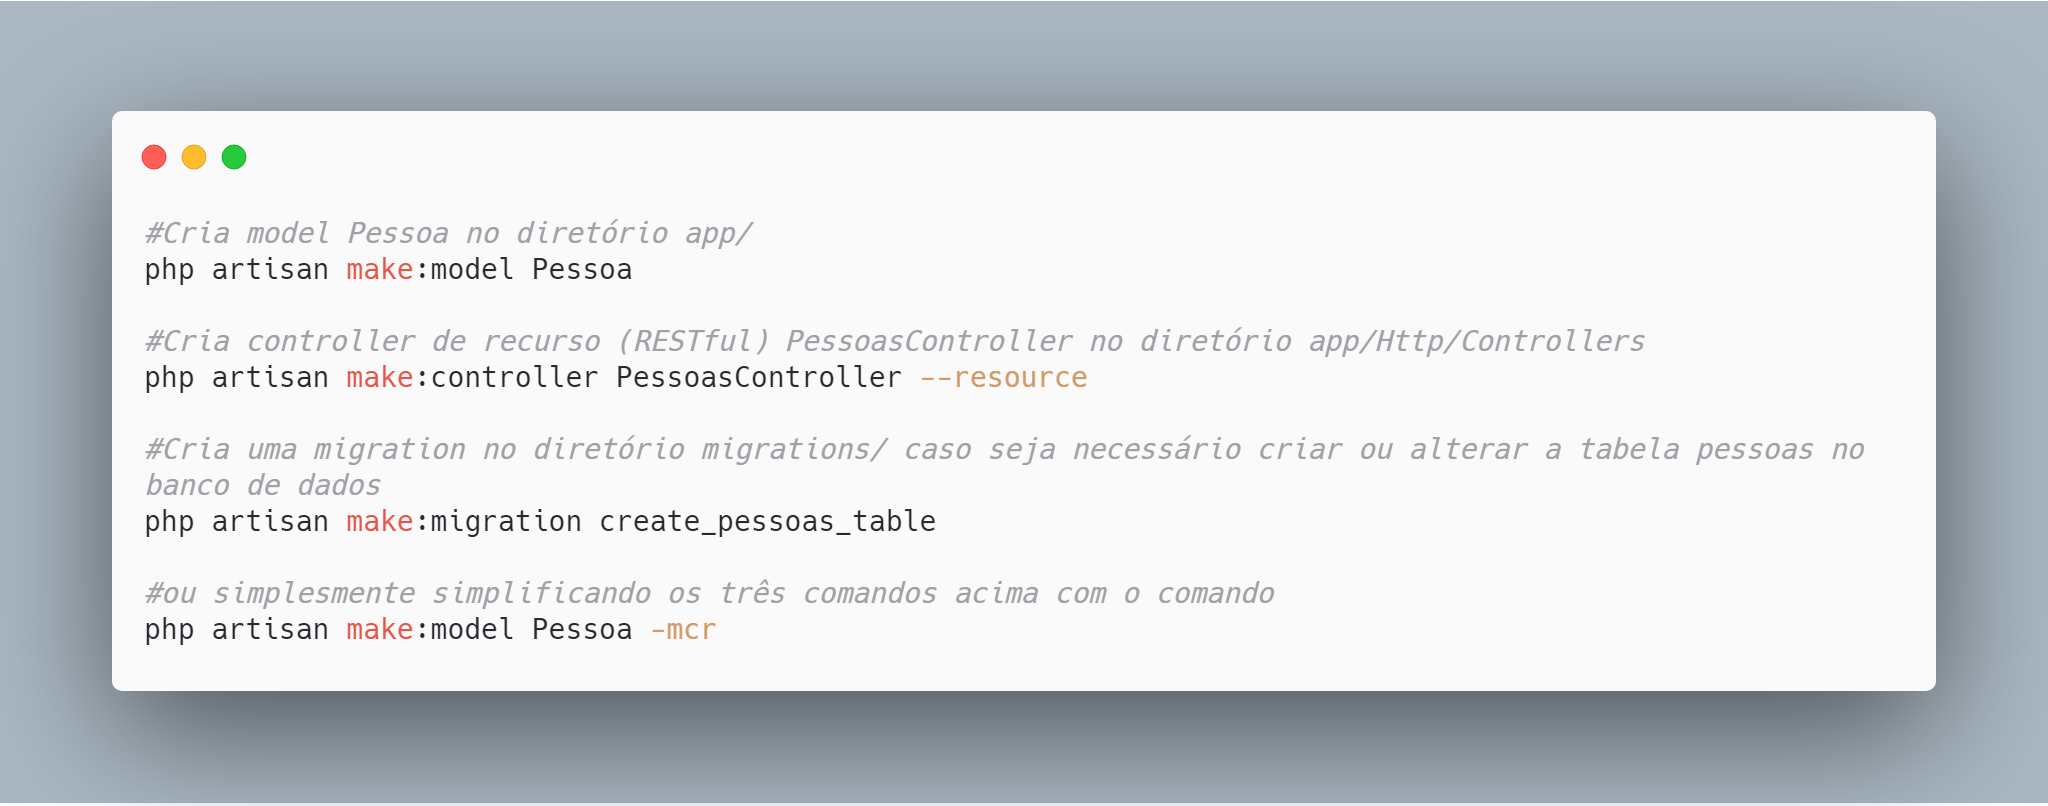
\includegraphics[width=13cm]{dados/figuras/php_artisan_make_model.png}
    \label{fig:artisanModel}
    \fonte{Autoria própria}
\end{figure}

O código fonte deste \textit{framework} se encontra no GitHub e possui cerca de 52.500 \textit{stars} ou \textit{likes}, e aproximadamente 500 contribuidores, sendo o framework backend, independente da linguagem, mais aclamado pelos desenvolvedores no mundo.

Algumas de suas principais características são a simplicidade da documentação e do motor de roteamento, o poderoso \textit{container} de injeção de dependências, suporte a múltiplos SGBD para armazenamento de sessões e \textit{cache}, um ORM intuitivo e expressivo, agnosticismo quanto SGBD para as migrações do sistema, o robusto suporte a tarefas agendadas em \textit{background} e transmissão de eventos em \textit{broadcast}.

\subsection{MVC com o Laravel}
\label{sub:mvclaravel}

A camada de \textit{model} do MVC é implementada no Laravel por meio do Eloquent ORM, que é uma implementação simples e amigável do padrão Active Record. Na \autoref{fig:modelEloquent} podemos observar as facilidades que este Object-Relational Mapper (ORM) traz para a manipulação de dados. Por padrão, os \textit{models} em uma aplicação desenvolvida com o Laravel se encontram no diretório \textit{app}.

\begin{figure}[H]
    \centering
    \caption{Exemplo de operações de busca usando o Eloquent ORM}
    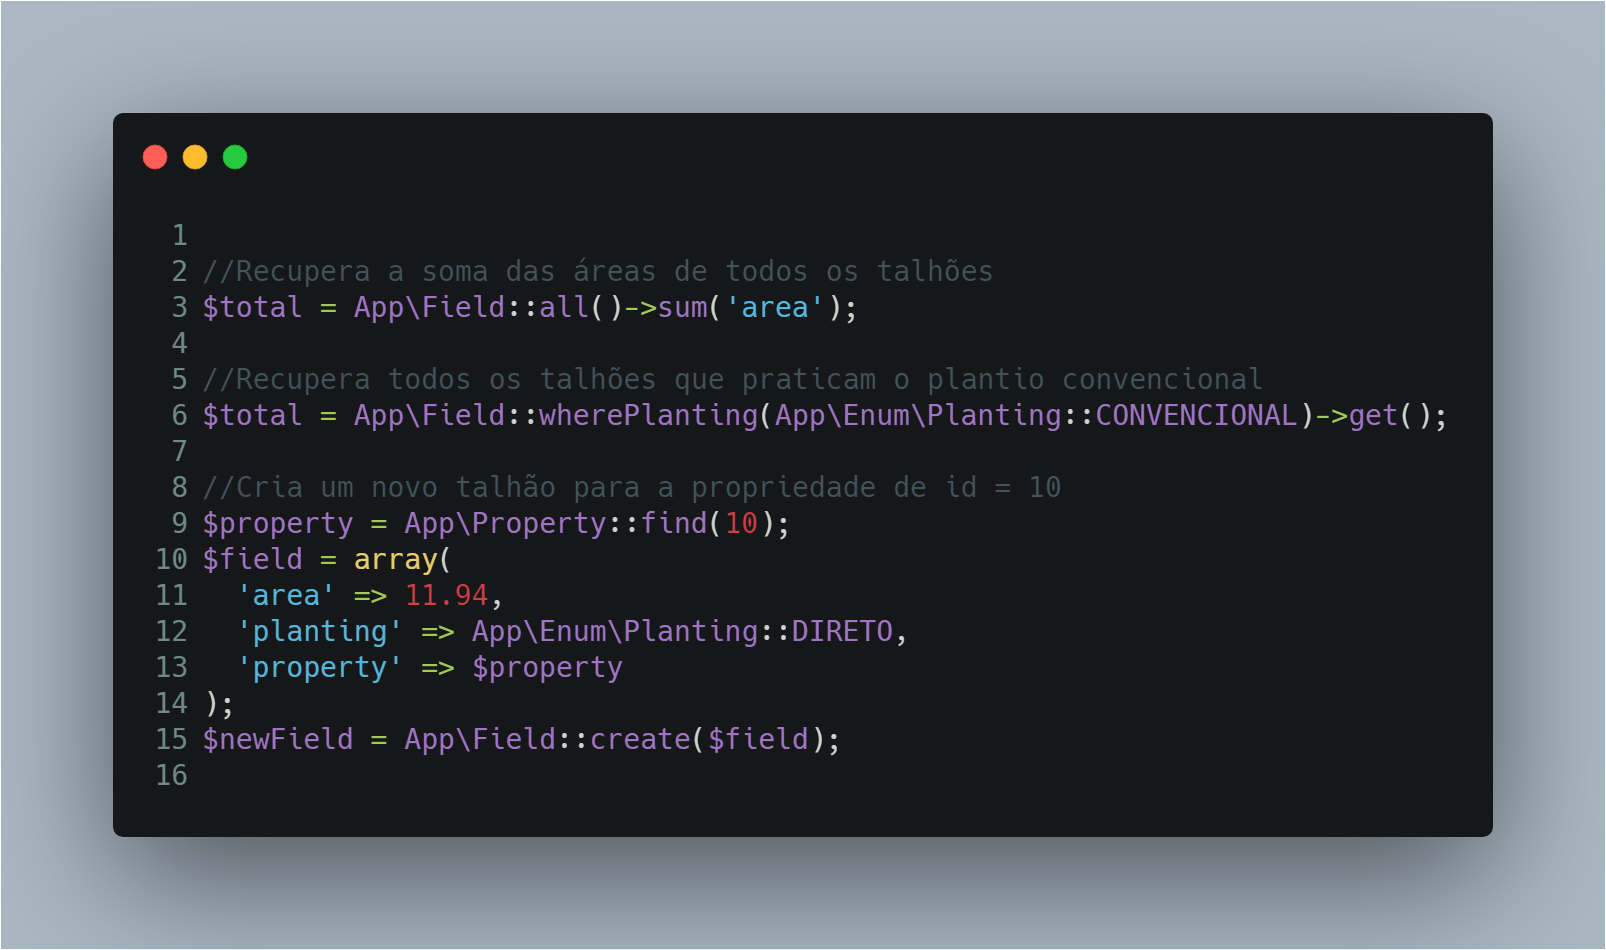
\includegraphics[width=13cm]{dados/figuras/exemplo_Model_Eloquent.png}
    \label{fig:modelEloquent}
    \fonte{Autoria própria}
\end{figure}

Na \autoref{fig:exemploRotas} é possível observar um exemplo de roteador utilizado no Laravel. O roteador é usado para determinar como será tratada uma requisição, dependendo de sua URI e verbo HTTP. No exemplo da \autoref{fig:exemploRotas}, é possível identificar quatro rotas possíveis no sistema. As chamadas são feitas usando a classe \textit{Route}, seguido de um método estático que representa o verbo HTTP da requisição, que recebe como o primeiro parâmetro a URI e no segundo o \textit{controller} seguido de um arroba e o nome do método que deverá tratar aquela requisição.

\begin{figure}[H]
    \centering
    \caption{Exemplo de roteador no Laravel}
    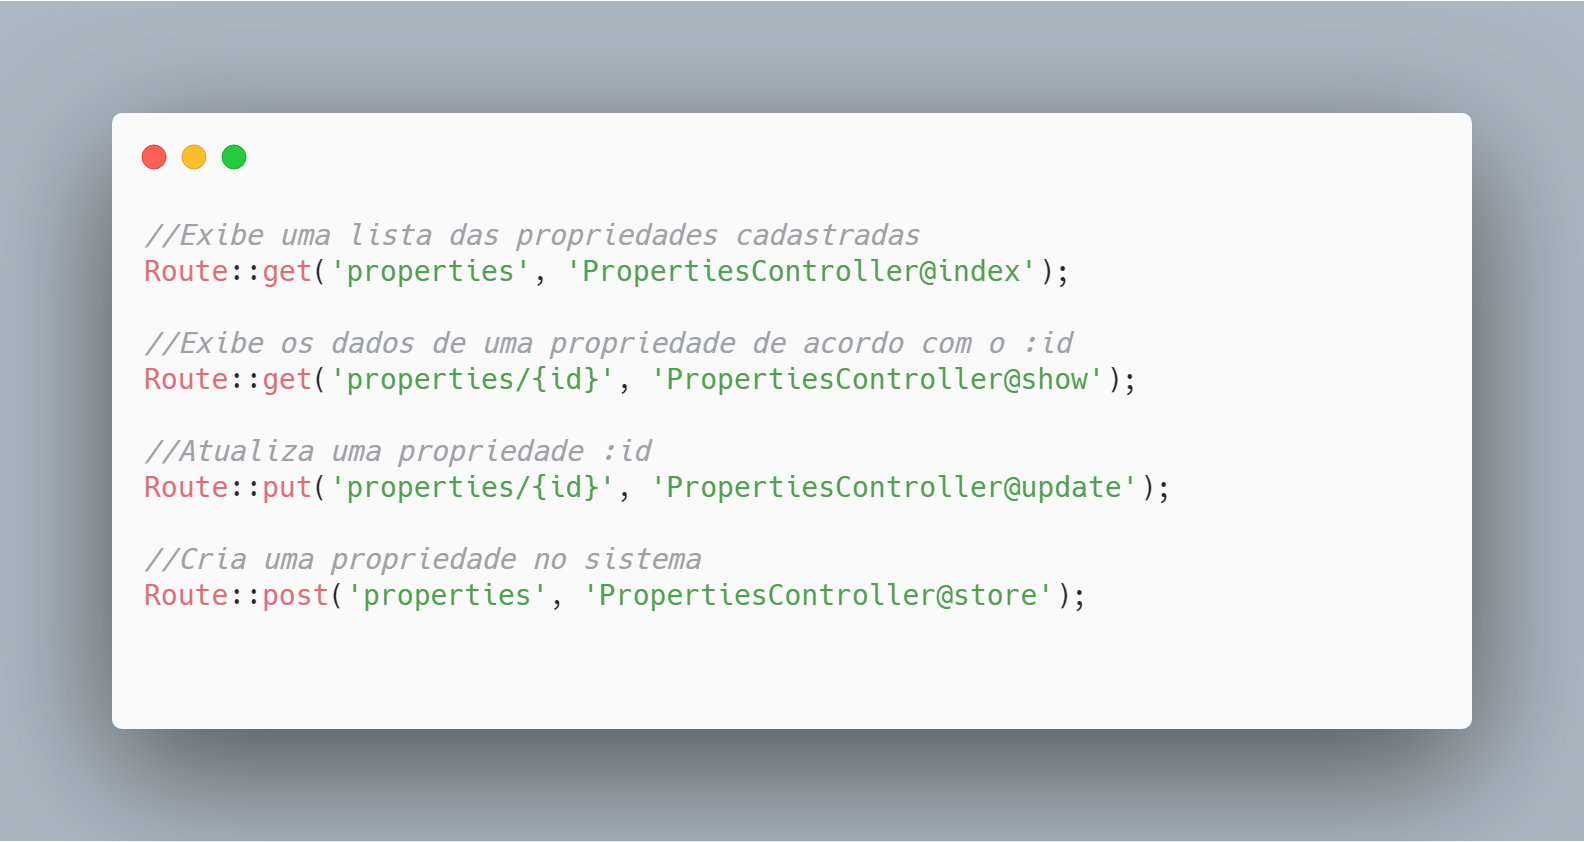
\includegraphics[width=13cm]{dados/figuras/exemplo_Rotas_Laravel.png}
    \label{fig:exemploRotas}
    \fonte{Autoria própria}
\end{figure}


No Laravel, por padrão, as classes \textit{controllers} se encontram no diretório App/Http/Controllers. Uma classe \textit{controller} no no Laravel não pode ser acessada diretamente, devendo o desenvolvedor criar rotas para este fim.

Na \autoref{fig:exemploController} é possível observar um exemplo de \textit{controller} no Laravel. O método \emph{store} é chamado quando uma requisição \emph{POST} é feita para a URI \emph{/properties}. Ao receber a requisição primeiramente é feita a validação dos dados e depois a criação do recurso na base de dados e então o usuário é redirecionada à listagem de propriedades.

\begin{figure}[H]
    \centering
    \caption{Exemplo de controller no Laravel}
    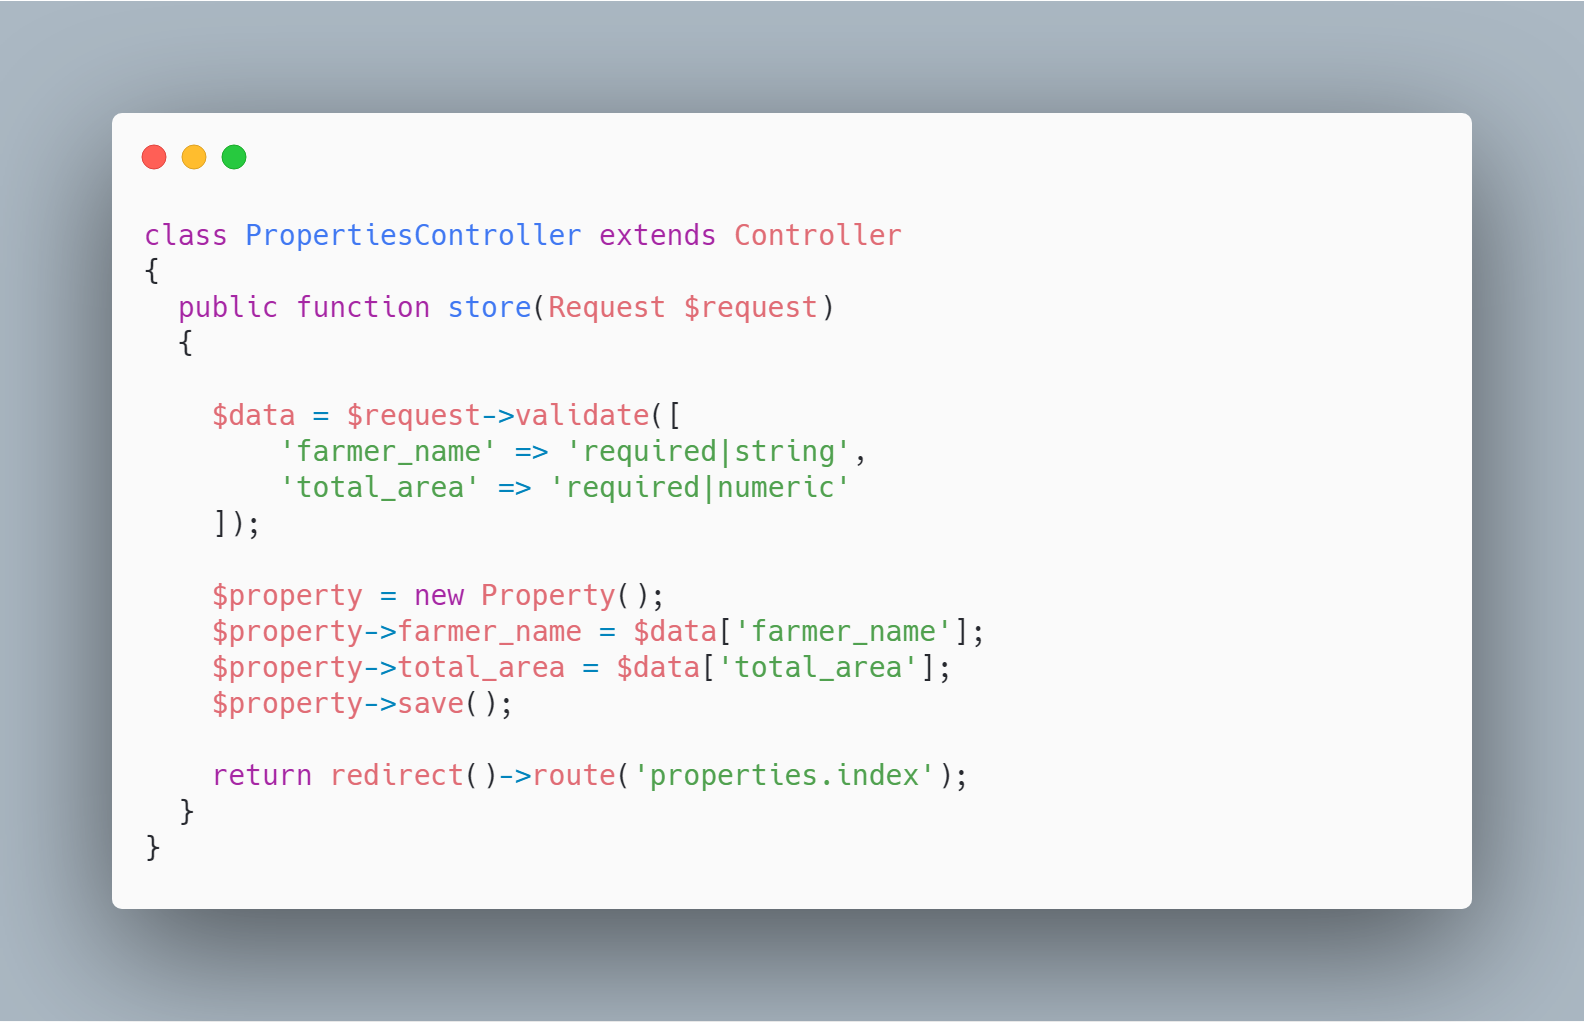
\includegraphics[width=13cm]{dados/figuras/exemplo_Controller_Laravel.png}
    \label{fig:exemploController}
    \fonte{Autoria própria}
\end{figure}

No desenvolvimento da presente aplicação a camada de \textit{view} não será implementada com o Laravel, sendo então repassada a responsabilidade de renderizar as informações no navegador para o React, descrito na \autoref{sub:react}.

\subsection{React}
\label{sub:react}

É uma biblioteca JavaScript mantida pela Facebook Inc. destinada principalmente à grandes aplicações, como o Facebook e Instagram, que devem atualizar uma grande quantidade de informações na tela em poucos segundos.

Essa biblioteca foi escolhida devido a característica da aplicação que deverá reagir aos inputs do usuário no formulário, informando os percentuais ideais de cada indicador químico na CTC, por exemplo. Além disso, possui uma documentação de fácil compreensão e uma das maiores comunidades, com milhares de perguntas e respostas para as mais diversas situações no StackOverflow e um repositório no GitHub com aproximadamente 130 mil \textit{stars} e 1300 contribuidores. 

A \autoref{fig:exemploViewReact} demonstra um exemplo de um componente do React. 

\begin{figure}[H]
    \centering
    \caption{Exemplo de componente com React}
    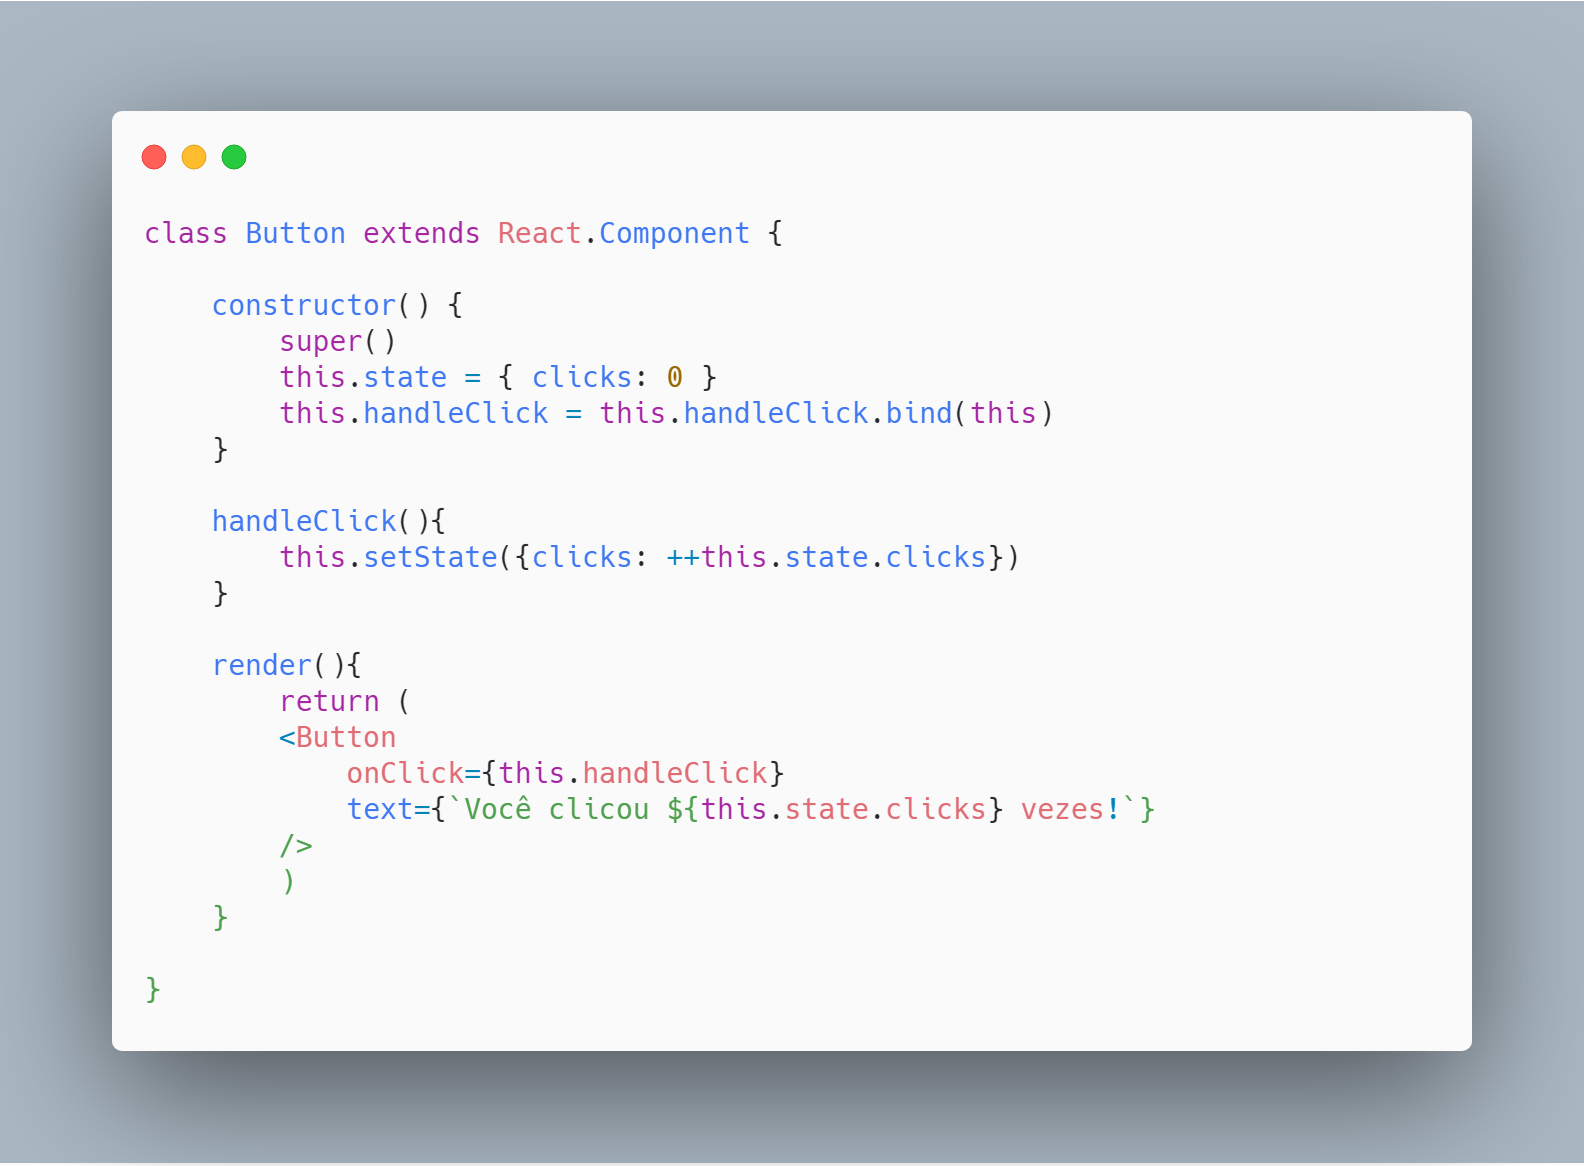
\includegraphics[width=13cm]{dados/figuras/exemplo_react_component.png}
    \label{fig:exemploViewReact}
    \fonte{Autoria própria}
\end{figure}

A \autoref{fig:exemploViewReact} apresenta o código JavaScript de um componente Button usando React. Esse código renderiza um botão que exibe um texto informando o usuário de quantas vezes aquele elemento foi clicado.

\subsection{Ant Design of React}
\label{sub:ant}

O Ant Design for React é uma biblioteca de componentes de interface para o React que pode ser requerida ao projeto por meio de um gerenciador de dependências como o Node Package Manager ou o Yarn. Ela fornece um conjunto de componentes de alta qualidade para o desenvolvimento de aplicações \textit{web}.

\subsection{Codeception}
\label{sub:codeception}

Para a escritas de teste de integração e unitários será utilizado o Codeception, um \textit{framework} para testes escrito em PHP que tem como objetivo facilitar a automação de testes em todas as camadas de um software.

Na \autoref{fig:excodeception} pode ser observado a facilidade de leitura e escrita de um teste de inusando Codeception.

\begin{figure}[H]
    \centering
    \caption{Exemplo de teste escrito com o Codeception}
    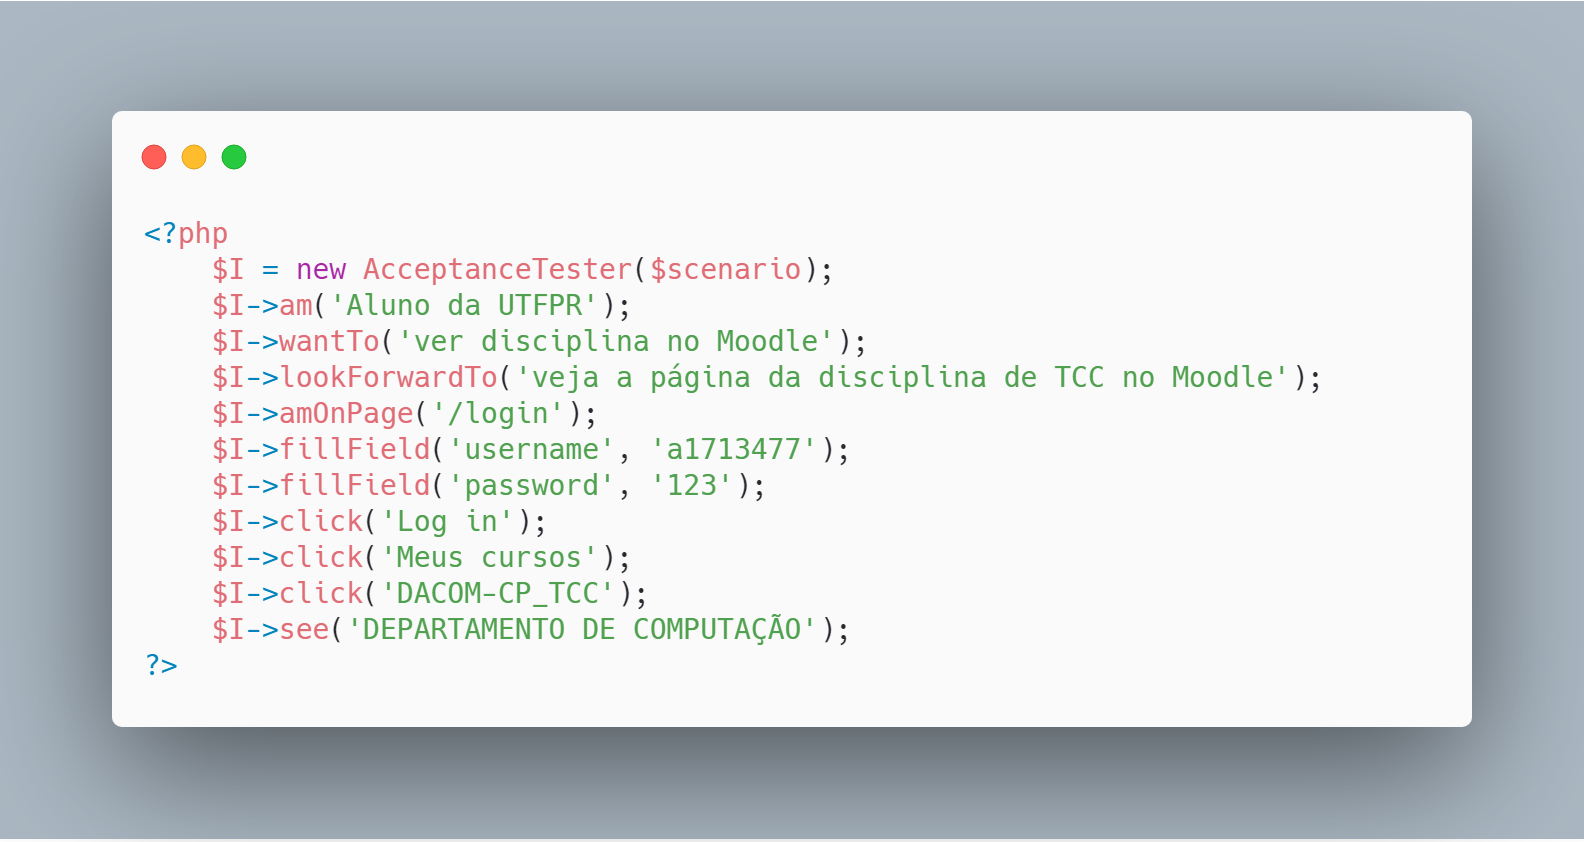
\includegraphics[width=13cm]{dados/figuras/teste_codeception.png}
    \label{fig:excodeception}
    \fonte{Autoria própria}
\end{figure}

\section{FERRAMENTAS}
\label{sec:ferramentas}
Nesta sessão serão apresentadas as ferramentas que serão úteis para o desenvolvimento e gerenciamento do projeto.

\subsection{Astah Community}
\label{sub:astah}

A ferramenta Astah Community é uma excelente ferramenta para modelagem UML. Por ser uma versão gratuita, possui algumas limitações. Apesar disso, essa versão satisfaz às necessidades do projeto visto que oferece suporte para a criação dos diagramas de caso de uso, classe e implantação.

\subsection{Trello}
\label{sub:trello}

O Trello é uma ferramenta de gerenciamento de projetos, simples e intuitiva baseada no conceito de kanban, recomendada para o gerenciamento de tarefas tanto individual quanto de equipes \cite{cardosopedro2016}.

Os projetos no Trello são representados por quadros. Dentro de cada quadro temos as listas, que aglomeram cartões. A menor configuração de listas recomendada em um projeto são em três listas: A fazer, fazendo e feito. Cada cartão representa uma tarefa e pode ser movido de uma lista para outra de acordo com o estado da tarefa.

Os cartões possuem diversas características, dentre as quais se destacam o prazo para conclusão, o rótulo, a possibilidade de criar \textit{checklists}, anexos e comentários.

\subsection{MySQL Workbench}
\label{sub:workbench}

O MySQL Workbench é uma ferramenta gratuita para a modelagem de dados, que auxilia os desenvolvedores na criação de modelos e administração de banco de dados MySQL. Ela possui diversas características muito úteis como a engenharia reversa e sincronização entre bases de dados.

Além disso, o Workbench é multiplataforma, oferecendo a aplicação nos ambientes Widnows, Linux e Mac OS. Ela fornece aos usuários diversas ferramentas para modelagem de banco de dados, realização de consultas com SQL e administração de banco.

\subsection{Visual Studio Code}
\label{sub:vscode}

O Visual Studio Code é uma ferramenta gratuita, de código aberto, que tem ganhado grande importância no cenário de desenvolvimento de software. Ela possui suporte a diversas linguagens de programação, dentre as quais o PHP e JavaScript, que serão as linguagens essenciais para a construção da aplicação.

\subsection{Git}
\label{sub:git}

A aplicação será versionada por meio do Git e terá o código-fonte hospedado no GitHub. O Git é um sistema de controle de versão de arquivos. Com ele é possível desenvolver projetos distribuídos de forma que toda alteração no código fonte é acompanhada. Com isso, vários desenvolvedores podem trabalhar no mesmo projeto sem risco de alterações. Sem o controle de versão, o desenvolvimento de aplicações se torna caótico.

\begin{figure}[H]
    \centering
    \caption{Demonstração do comportamento das \textit{branchs} no repositório Git}
    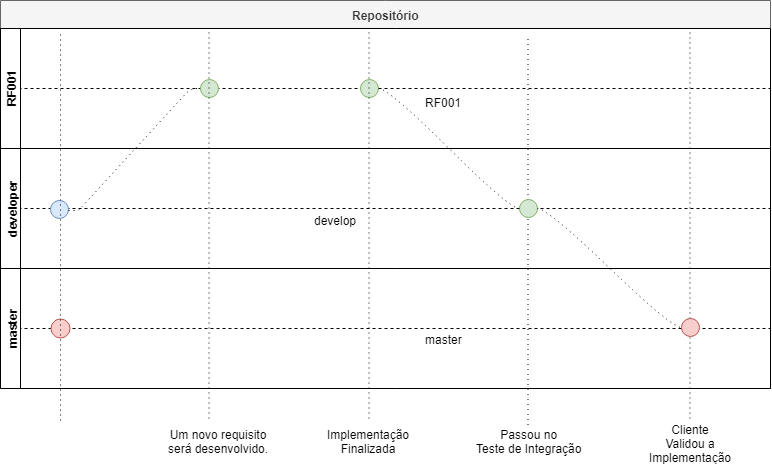
\includegraphics[width=13cm]{dados/figuras/git.png}
    \label{fig:exemplogit}
    \fonte{Autoria própria}
\end{figure}

Conforme exemplificado na \autoref{fig:exemplogit}, o repositório será divido em duas \textit{branches} principais: \textit{developer} e \textit{master}. A \textit{master} será a versão utilizada para a aplicação em produção. Enquanto a \textit{developer}, para o ambiente de homologação.

Quando uma nova funcionalidade precisa ser desenvolvida, é criada uma \textit{branch} específica a partir da versão de homologação. Após a conclusão da tarefa o desenvolvedor deve fazer um \textit{pull request} ou \textit{merge request} para a versão de homologação.

Caso tenha passado pelos testes e aprovada pelo cliente, então essa nova versão de homologação deverá ser unida com a master, gerando assim uma nova versão da aplicação. Após isso, o desenvolvedor deverá executar o \textit{pull} no servidor para versão de produção seja atualizada.

\section{METODOLOGIA}
\label{sec:metodologiadev}

Neste capítulo será apresentada a metodologia para o desenvolvimento da aplicação. Como o desenvolvimento da aplicação será realizado apenas por um desenvolvedor, fica inviável seguir um processo de software. Com isso, foi necessário uma adaptação de um modelo existente para o presente projeto. O modelo desenvolvido segue alguns traços do modelo iterativo-incremental, pois dos modelos consolidados disponíveis é o que mais se adéqua às mudanças no projeto, além de ser o modelo adotado pelo Scrum que influenciou a modelagem deste processo.

\subsection{Processo}
\label{sub:processo}
Nesta seção será explicada a \autoref{fig:modeloprocesso}, o fluxo dos requisitos do sistema desde a fase de análise até chegar na etapa de implementação.

\begin{figure}[H]
    \centering
    \caption{Modelo de aplicação do TDD no projeto}
    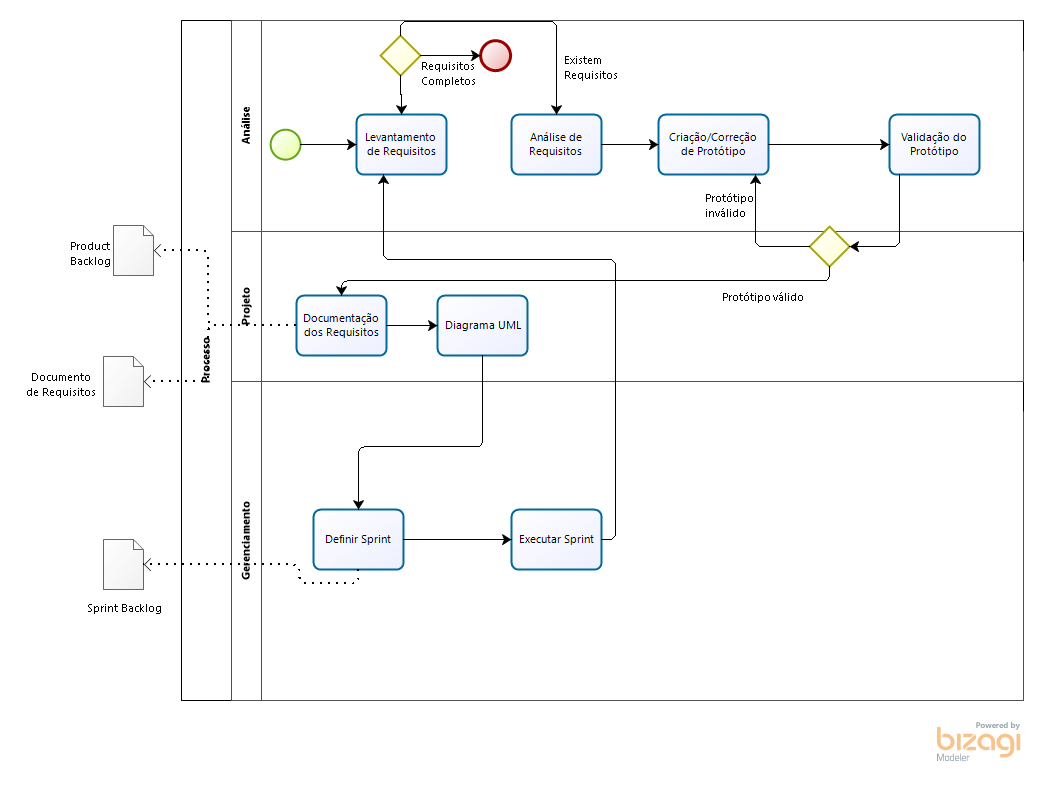
\includegraphics[width=13cm]{dados/figuras/ModeloDoProcesso.png}
    \label{fig:modeloprocesso}
    \fonte{Autoria própria}
\end{figure}

Primeiramente, é necessário o levantamento do requisitos, que é a etapa na qual o desenvolvedor deve entender qual é a necessidade do cliente. Existem diversos métodos para este fim, porém no presente projeto foi utilizado análise de documentos, no caso da planilha usado nos cálculos. Análise de requisitos foi feita em conjunto com o orientador, pois representa o cliente no projeto assim como o desenvolvimento dos protótipos. 

Após a análise foi iniciada a fase de projeto, Com os protótipos construídos, é dado início a etapa de documentação dos requisitos funcionais e não funcionais, além da especificação. Logo após, os diagramas da UML foram desenvolvidos, servindo de subsídios para a próxima fase.

Já na fase de gerenciamento são definidas as \textit{sprints}, formando o \textit{Sprint backlog} da próxima iteração da fase de implementação, descrita na \autoref{subsec:tdd}, que tem como entrada este artefato.

\subsection{Kanban}
\label{subsec:kanban}

Para o gerenciamento de tarefas, será utilizado o conceito de quadros \textit{kanban}, utilizando a ferramenta Trello. As tarefas serão divididas em seis quadros, demonstrados na \autoref{fig:trelloquadro}, que são:

\begin{itemize}
    \item \textbf{\textit{Product backlog}}: Os requisitos que foram definidos para o produto
    \item \textbf{\textit{Sprint backlog}}: Os requisitos que devem ser desenvolvidos na \textit{sprint} atual
    \item \textbf{\textit{Doing}}: Os requisitos que estão sendo desenvolvidos no momento
    \item \textbf{\textit{Done}}: Os requisitos que foram finalizados
    \item \textbf{\textit{Test}}: Os requisitos que após a finalização, foram enviados para teste em um servidor de homologação.
    \item \textbf{\textit{Deploy}}: Os requisitos que foram homologados e podem ir para produção.
\end{itemize}

\begin{figure}[H]
    \centering
    \caption{Quadro \textit{kanban} do projeto}
    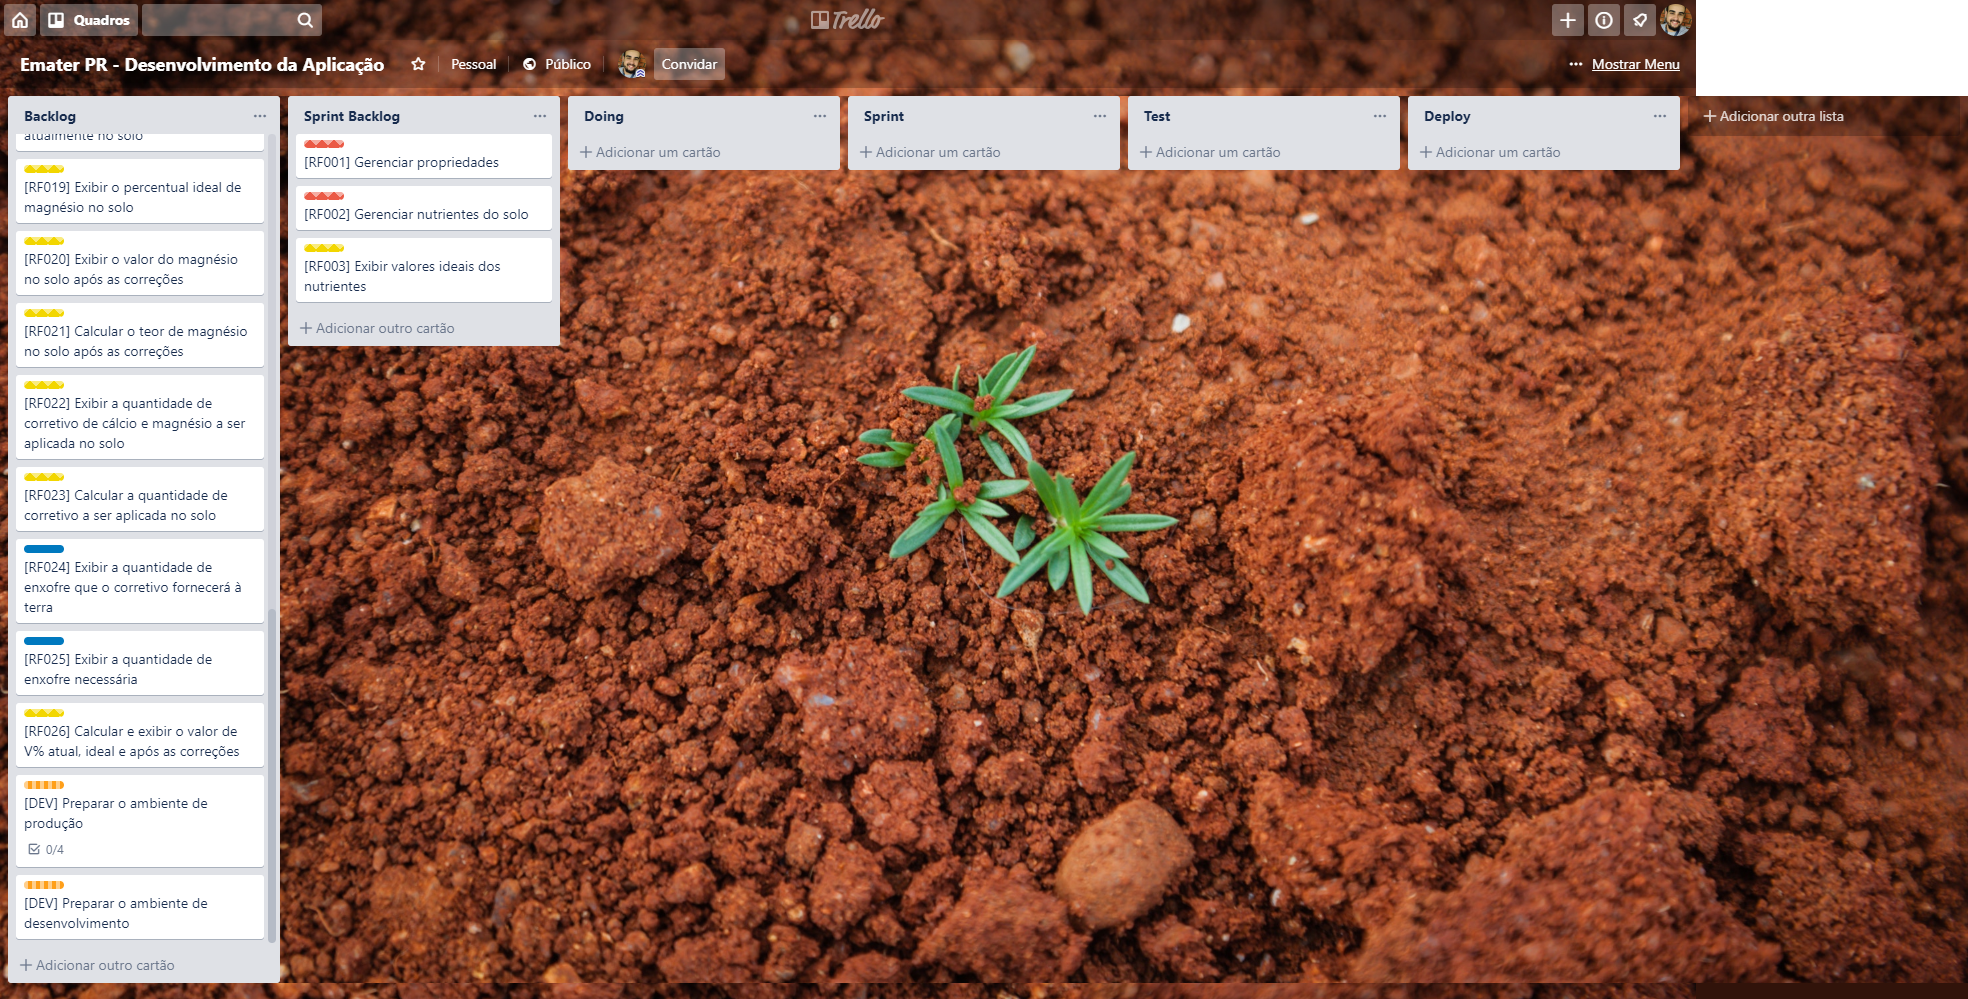
\includegraphics[width=13cm]{dados/figuras/quadro_trello.png}
    \label{fig:trelloquadro}
    \fonte{Autoria própria}
\end{figure}

\subsection{Test Driven Development}
\label{subsec:tdd}

Para aumentar a confiabilidade e a qualidade, um sistema requer a presença de testes automatizados \cite{myers2004art}. Devido a esse fato, o sistema será desenvolvidos seguindo os princípios do \textit{Test} \textit{Driven} \textit{Development} (TDD). Esta técnica tem como principal característica a escrita do teste antes da implementação da funcionalidade, sendo assim, há uma inversão de lógica quando comparamos aos modelos tradicionais \cite{erdogmus2005effectiveness}. A geração de testes antes da implementação da funcionalidade auxilia no desenvolvimento de sistemas mais bem estruturados, com menos problemas e mais flexíveis \cite{melnik2007empirical}.

Neste ciclo, cada iteração possui três momentos. O primeiro é o \textit{red}, no qual o teste é escrito e, como a funcionalidade ainda não está implementada, o teste deve falhar. O próximo passo é o \textit{green}, no qual a funcionalidade é escrita sem se preocupar com os conceitos de \textit{clean} \textit{code}, tendo como único objetivo passar no teste. Após passar pelo teste, o código implementado deve ser refatorado (\textit{refactor}), procurando se adequar aos padrões de código para garantir a legibilidade e a correta organização desse trecho.

Este técnica, segundo \citeonline{aniche2014test}, pode ser vantajosa para seus praticantes. Dentre essas vantagens destacam-se:

\begin{itemize}
    \item Começando pelo teste, o programador consegue pensar somente no que o código deve fazer, e assim sendo, esquece por instantes da implementação. Isso ajuda ao programador pensar nos melhores casos de teste para o trecho em desenvolvimento.
    \item Se seguido corretamente durante todo o processo de desenvolvimento, todo o código deverá ter pelo menos um teste de unidade atestando que este funciona corretamente.
    \item Como o programador deve buscar pela solução mais simples, acabará escapando de soluções complexas, muitas vezes desnecessárias.
    \item Muitas vezes o desenvolvedor tradicional gera um acoplamento ou desconexão entre as classes devido ao pensamento somente na classe que está trabalhando em um determinado momento. Porém, quando o teste é desenvolvido antes, o desenvolvedor pensa sobre como o código que está testando deve se comportar perante os outros e com isso pode tomar decisões mais inteligentes, gerando um maior reaproveitamento de código além de nomes de classes, atributos, métodos, parâmetros e retorno com nomes mais intuitivos, trazendo uma melhor qualidade ao código. 
    \item O desenvolvedor sempre está recebendo \textit{feedbacks} sobre o estado do código que foi desenvolvido, enquanto no modelo tradicional esses \textit{feedbacks} só serão gerados após o desenvolvimento de vários trechos de código.
\end{itemize}

Em suma, o TDD potencializa a quantidade de \textit{feedback} sobre o código que está sendo gerado, fazendo o programador reconhecer os defeitos antecipadamente, diminuindo o retrabalho e os custos de manutenção e aumentando a qualidade do código. 

Na figura \autoref{fig:ciclotdd}, é exemplificado o ciclo do TDD no desenvolvimento dessa aplicação.

\begin{figure}[H]
    \centering
    \caption{Modelo de aplicação do TDD no projeto}
    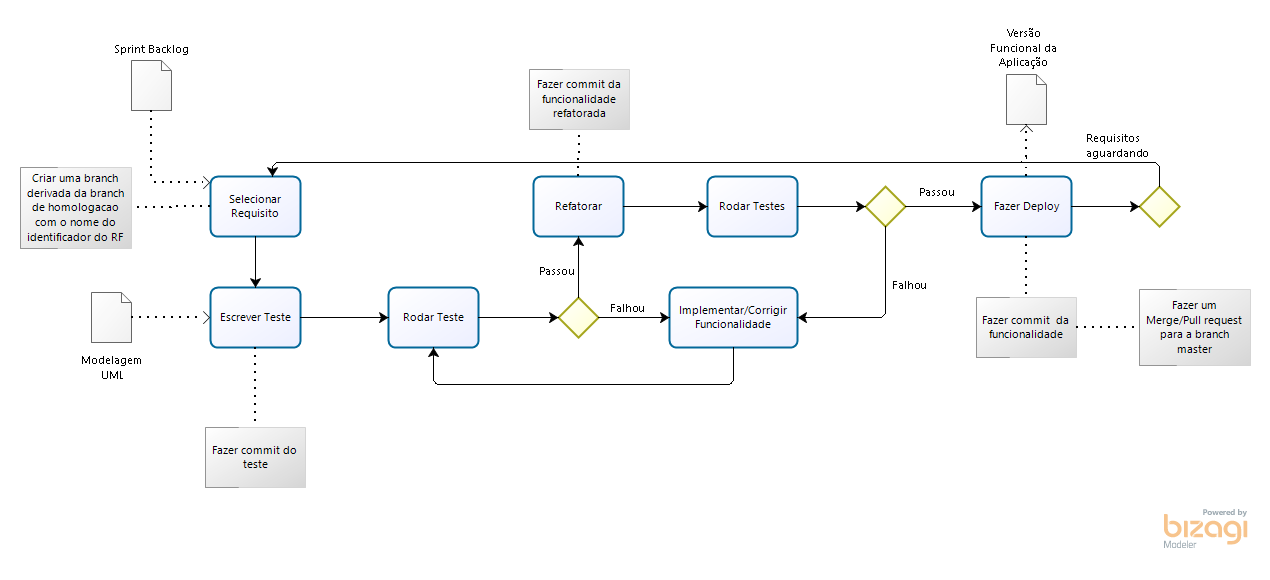
\includegraphics[width=13cm]{dados/figuras/ModeloDeAplicacaoTDD.png}
    \label{fig:ciclotdd}
    \fonte{Autoria própria}
\end{figure}

O modelo apresentado na \autoref{fig:ciclotdd} representa as etapas de uma \textit{Sprint}. É possível observar que na primeira etapa o desenvolvedor seleciona um requisito do \textit{Sprint backlog} e cria uma \textit{branch} para trabalhar nessa funcionalidade, logo após, ele deve escrever um teste, fazer um \textit{commit} então executar o teste que falhará, pois neste momento a funcionalidade ainda não foi implementada. Então, o usuário deverá seguir para a etapa de Implementação/Correção de Funcionalidade. Após concluir, deverá executar novamente o teste. Neste momento, caso o teste passe, deverá seguir para a etapa de refatoração. Após a refatoração o programador deve executar os testes de integração para ver se a nova funcionalidade se encaixou sem quebrar o sistema. Caso passe nos testes, essa funcionalidade deverá ser marcada com \textit{commit} e então enviada para \textit{deploy} no servidor de homologação para aprovação. Caso aprovado o código será incluído no servidor de produção.

O controle do estado de cada requisito será feito usando o Trello, utilizando o conceito de Kanban. Após todos os requisitos passarem pelo processo, a aplicação deve estar totalmente funcional, executando todas as tarefas que foram enumeradas na \autoref{rf:tabela}.

\section{ARQUITETURA DO SOFTWARE}
\label{sub:arquitetura}

O presente projeto seguirá o padrão arquitetural Model-View-Controller (MVC), este que \citeonline{da2012revisao} sugere uma arquitetura de software dividida em componentes, de tal forma que o código fique mais limpo e organizado, o que favorece o reaproveitamento de código e fornece uma manutenção mais segura. Porém, para que haja a independência entre os componentes, deve haver uma organização do sistema em camadas, garantindo a facilidade de escala, reuso e eficiência.

A camada \textit{model} é responsável por tratar a manipulação e persistência de dados internos, comunicando, sobretudo, com o armazenamento de dados.

Já a camada \textit{controller} é responsável pelo intermédio entre as ações que o usuário executa na interface (\textit{View}) e a resposta do servidor para essa ação, que normalmente é entregue por \textit{model}. 

Finalmente, a camada \textit{view} representa a interface pela qual o usuário interage com a aplicação. Ela define o formato de renderização mais adequado para a resposta de uma requisição.

\section{CRONOGRAMA DO PROJETO}
\label{sec:cronograma}

O gráfico abaixo representa o cronograma do projeto. O desenvolvimento será divido em sprints, que serão 

O gráfico do abaixo demonstra a distribuição das atividades do projeto em relação ao tempo. A data da primeira reunião com o professor orientador foi considerada a data inicial do cronograma, na qual foi definido o tema a ser desenvolvido. A duração de cada atividade está na unidade de dias.

\begin{landscape}

    \begin{ganttchart}
        [
            y unit title=0.4cm,
            y unit chart=0.5cm,
            vgrid,hgrid,
            title height=1,
            bar/.style={draw,fill=green},
            bar incomplete/.append style={fill=yellow!50},
            bar height=0.7
        ]{1}{36}

        \gantttitle{Junho}{6}
        \gantttitle{Julho}{5}
        \gantttitle{Agosto}{5}
        \gantttitle{Setembro}{5}
        \gantttitle{Outubro}{5}
        \gantttitle{Novembro}{5}
        \gantttitle{Dezembro}{5} \\

        \gantttitlelist{1,...,6}{1}
        \gantttitlelist{1,...,5}{1}
        \gantttitlelist{1,...,5}{1}
        \gantttitlelist{1,...,5}{1}
        \gantttitlelist{1,...,5}{1}
        \gantttitlelist{1,...,5}{1}
        \gantttitlelist{1,...,5}{1} \\

        \gantttitlelist{1,...,36}{1} \\

        \ganttbar{Desenvolvimento da Interfaces}{2}{17} \\

        \ganttbar{Desenvolvimento da API Rest}{4}{20} \\

        \ganttbar{Correções no Documento}{5}{5}
        \ganttbar{}{10}{10}
        \ganttbar{}{15}{15}
        \ganttbar{}{20}{20}
        \ganttbar{}{24}{30}\\

        \ganttbar{Entrega do Documento}{31}{30} \\

        \ganttbar{Validação pelo técnico}{5}{4}
        \ganttbar{}{10}{9}
        \ganttbar{}{15}{14}
        \ganttbar{}{20}{19} \\

        \ganttbar{Entrega parcial}{7}{6}
        \ganttbar{}{12}{11}
        \ganttbar{}{17}{16}
        \ganttbar{}{22}{21} \\

        \ganttbar{Implantação}{22}{24} \\

        \ganttbar{Testes exploratórios pelo cliente}{25}{29} \\
        \ganttbar{Correção de bugs}{25}{29} \\

    \end{ganttchart}

\end{landscape}
                   % Proposta
% REQUISITOS------------------------------------------------------------------

\chapter{ANÁLISE E PROJETO DO SISTEMA}
\label{chap:analise}
Neste capítulo serão exibidos os Requisitos Funcionais e Não Funcionais, bem como a Especificação dos Requisitos Funcionais, o Diagrama de Casos de Uso Geral, o Diagrama de Classes e o Diagrama Entidade-Relacionamento.

\subsection{Requisitos Funcionais}
\label{sec:titSecReqFunc}

Os requisitos funcionais são artefatos gerados pela especificação de requisitos, que é o processo de escrever os requisitos de usuário e de sistema em um documento de requisitos. Preferencialmente, os requisitos de usuário e sistema devem ser claros, inequívocos, de fácil compreensão, completos e consistentes. Porém, na prática, é difícil que isso ocorra, visto que os envolvidos no processo veem os requisitos de formas diferentes, e em grande parte das vezes, nota-se conflitos e inconsistências relacionadas à esses requisitos \cite{Sommerville10}.

No presente projeto os requisitos foram obtidos com base na planilha de cálculo de correção e equilíbrio do solo, fornecida pelo cliente, utilizando a técnica de etnografia, que consiste em uma técnica de observação que pode ser usada na elicitação e análise de requisitos. O etnógrafo imerge no ambiente dos usuários e observa os hábitos de seu trabalho diário. Os requisitos de software podem ser deduzidos a partir dessas observações \cite{Sommerville10}.

\begin{landscape}
\begin{longtable}{|p{1.5cm}|p{5cm}|p{9cm}|p{2.5cm}|}
    \hline
    ID    & REQUISITO                                                                        & DESCRIÇÃO                                                                                                                                                                                                                                                                                               & PRIORIDADE \\\hline
    \endfirsthead
    %
    \hline
    ID    & REQUISITO                                                                        & DESCRIÇÃO                                                                                                                                                                                                                                                                                               & PRIORIDADE \\\hline
    \endhead
    %
    RF001 & Gerenciar informações da propriedade.                                            & O sistema deve permitir ao usuário cadastrar, remover, alterar ou listar informações do solo de um produtor.                                                                                                                                                                                            & Essencial  \\\hline
    RF002 & Gerenciar nutrientes do solo.                                                    & O sistema deve permitir ao usuário inserir, remover, alterar ou listar os nutrientes coletados na análise do solo.                                                                                                                                                                                      & Essencial  \\\hline
    RF003 & Exibir valores ideais.                                                           & O sistema deve exibir os valores ideais de cada teor inserido de acordo com a textura do solo.                                                                                                                                                                                                          & Importante \\\hline
    RF004 & Exibir valores dos nutrientes após correções.                                    & O sistema deve exibir os valores dos nutrientes inseridos após as correções.                                                                                                                                                                                                                            & Importante \\\hline
    RF005 & Gerenciar matéria orgânica.                                                      & O sistema deve permitir ao usuário inserir, remover, alterar ou listar o teor da matéria orgânica (M.O.) do solo.                                                                                                                                                                                       & Essencial  \\\hline
    RF006 & Exibir teor ideal da M.O.                                                        & O sistema deve exibir o teor ideal de matéria orgânica (M.O.).                                                                                                                                                                                                                                          & Importante \\\hline
    RF007 & Gerenciar dados relacionados à correção/recuperação  de Fósforo.                 & O sistema deve permitir ao usuário cadastrar, remover,  alterar ou listar valores ligados ao Fósforo, tais como teor a ser atingido, fonte a ser utilizada e eficiência.                                                                                                                                & Essencial  \\\hline
    RF008 & Exibir valores a serem aplicados no processo de correção/recuperação de Fósforo. & O sistema deve informar ao usuário a quantidade de Fósforo à ser aplicada assim como o seu custo.                                                                                                                                                                                                       & Importante \\\hline
    RF009 & Gerenciar valor/ton. (R\$) no processo relacionado às fontes de Fósforo.         & O sistema deve possibilitar ao usuário inserir, remover, alterar ou listar valores relacionados às fontes: superfosfato simples, superfosfato triplo, MAP, DAP, Yoorin, Fosfato Arad, Fosfato Gafsa, Fosfato Daoui, Fosfato  Patos Minas, Escória de Thomas, ácido Fosfórico e multifosfato magnesiano. & Essencial  \\\hline
    RF010 & Gerenciar dados relacionados à correção/recuperação do Potássio.                 & O sistema deve possibilitar ao usuário inserir, remover,  alterar ou listar dados relacionados à participação do Potássio na CTC assim como a fonte de Potássio a ser usada.                                                                                                                            & Essencial  \\\hline
    RF011 & Exibir valores relacionados à correção/recuperação do Potássio.                  & O sistema deve informar ao usuário dados à respeito do Potássio tais como: participação atual na CTC do solo,  participação do Potássio na CTC após correção, quantidade e custo a ser aplicada e sua participação ideal na CTC.                                                                        & Importante \\\hline
    RF012 & Gerenciar valor/ton. (R\$) no processo relacionado às fontes de Potássio.        & O sistema deve permitir ao usuário cadastrar, excluir, alterar ou listar valores como: cloreto de Potássio, Sulfato de Potássio e Sulfato de Potássio/Magnésio.                                                                                                                                         & Essencial  \\\hline
    RF013 & Cadastrar dados para a correção do cálcio e magnésio no solo                     & O sistema deve permitir o usuário informar dados acerca da correção do cálcio no solo.                                                                                                                                                                                                                  & Essencial \\\hline
    RF014 & Alterar dados para a correção do cálcio e magnésio no solo                       & O sistema deve permitir o usuário alterar os dados sobre a correção do solo.                                                                                                                                                                                                                            & Desejável  \\\hline
    RF015 & Exibir o teor de cálcio atualmente no solo                                       & O sistema deve apresentar ao usuário, o percentual de Cálcio na CTC atual (antes das correções)                                                                                                                                                                                                         & Essencial  \\\hline
    RF016 & Exibir o teor de cálcio ideal no solo                                            & O sistema deve apresentar ao usuário, o intervalo percentual de Cálcio ideal na CTC.                                                                                                                                                                                                                    & Importante  \\\hline
    RF017 & Calcular o percentual de cálcio ideal no solo                                    & O sistema deve apresentar ao usuário, o percentual ideal de Cálcio na CTC.                                                                                                                                                                                                                              & Importante  \\\hline
    RF018 & Exibir teor de magnésio atualmente no solo                                       & O sistema deve apresentar ao usuário o percentual de Magnésio atual na CTC.                                                                                                                                                                                                                             & Importante  \\\hline
    RF019 & Exibir o percentual ideal de magnésio no solo                                    & O sistema deve apresentar ao usuário o percentual de Magnésio ideal na CTC.                                                                                                                                                                                                                             & Importante  \\\hline
    RF020 & Exibir o valor do magnésio no solo após as correções                             & O sistema deve apresentar ao usuário o percentual de Magnésio na CTC após as correções.                                                                                                                                                                                                                 & Importante  \\\hline
    RF021 & Calcular o teor de magnésio no solo após as correções                            & O sistema deve calcular o percentual de Magnésio na CTC após as correções.                                                                                                                                                                                                                              & Importante  \\\hline
    RF022 & Exibir a quantidade de corretivo de cálcio e magnésio a ser aplicada no solo.    & O sistema deve exibir a quantidade a ser aplicada, em toneladas por hectare, do corretivo informado.                                                                                                                                                                                                    & Importante  \\\hline
    RF023 & Calcular a quantidade de corretivo a ser aplicada no solo.                       & O sistema deve calcular a quantidade a ser aplicada, em toneladas por hectare, do corretivo informado.                                                                                                                                                                                                  & Importante  \\\hline
    RF024 & Exibir a quantidade de enxofre que o corretivo fornecerá à terra                 & O sistema deve exibir o valor, em quilogramas por hectare, da quantidade de enxofre que o corretivo fornecerá.                                                                                                                                                                                          & Desejável  \\\hline
    RF025 & Exibir a quantidade de enxofre necessária                                        & O sistema deve exibir a quantidade suficiente, em quilogramas por hectare, da quantidade de enxofre necessária.                                                                                                                                                                                         & Desejável  \\\hline
    RF026 & Calcular e exibir o valor de V\% atual, ideal e após as correções                & O sistema deve calcular e exibir os valores de V\% atual, ideal e após as correções.                                                                                                                                                                                                                    & Importante  \\\hline
    \caption{Tabela de Requisitos Funcionais}
    \label{rf:tabela}
\end{longtable}
\end{landscape}

\clearpage

\begin{quadro}[!htb]
    \begin{tabular}{|p{3cm}|p{11cm}|}
        \hline
        \textbf{RS300} & \textbf{Cadastrar dados para a correção do cálcio e magnésio no solo} \\
        \hline
        Sumário        & O sistema deve permitir o usuário informar dados acerca da correção do cálcio no solo.                  \\
        \hline
        Pré-condições  & O usuário deve estar logado no sitema                  \\
        \hline
        Atores         & Usuário                  \\
        \hline
        Descrição      &
        \begin{itemize}
            \item Informa o percentual de cálcio desejado na CTC
            \item Seleciona qual fonte de cálcio será utilizada na correção
            \item Informa o custo médio em R\$/ha do corretivo
            \item Informa o percentual de PRNT do corretivo
            \item Informa o teor de CaO do corretivo
        \end{itemize}                 \\
        \hline
        Alternativas   &
        \begin{itemize}
            \item Caso o usuário não saiba o teor de CaO, será utilizado o valor médio do corretivo
        \end{itemize}                 \\
        \hline
        Exceção        &
        \begin{itemize}
            \item Caso o usuário informe um valor percental fora do intervalo de 0 a 100, não poderá proseguir com o preenchimento de outros campos.
            \item Caso o usuário informa um corretivo que não exista, uma mensagem de erro deverá ser exibida.
        \end{itemize}                   \\
        \hline
    \end{tabular}
\end{quadro}

\begin{quadro}[!htb]
    \begin{tabular}{|p{3cm}|p{11cm}|}
        \hline
        \textbf{RS301} & \textbf{Alterar dados para a correção do cálcio e magnésio no solo} \\
        \hline
        Sumário        & O sistema deve permitir o usuário alterar os dados sobre a correção do solo.                  \\
        \hline
        Pré-condições  & \begin{itemize}
            \item O usuário deve estar logado
            \item O usuário deverá acessar uma ??análise?? já existente 
        \end{itemize}                 \\
        \hline
        Atores         & Usuário                  \\
        \hline
        Descrição      &
        \begin{itemize}
            \item Informa o percentual de cálcio desejado na CTC
            \item Seleciona qual fonte de cálcio será utilizada na correção
            \item Informa o custo médio em R\$/ha do corretivo
            \item Informa o percentual de PRNT do corretivo
            \item Informa o teor de CaO do corretivo
        \end{itemize}                 \\
        \hline
        Alternativas   &
        \begin{itemize}
            \item Caso o usuário não saiba o teor de CaO, será utilizado o valor médio do corretivo
        \end{itemize}                 \\
        \hline
        Exceção        &
        \begin{itemize}
            \item Caso o usuário informe um valor percental fora do intervalo de 0 a 100, não poderá proseguir com o preenchimento de outros campos.
            \item Caso o usuário informe um corretivo que não exista, uma mensagem de erro deverá ser exibida.
        \end{itemize}                   \\
        \hline
    \end{tabular}
\end{quadro}

\begin{quadro}[!htb]
    \begin{tabular}{|p{3cm}|p{11cm}|}
        \hline
        \textbf{RS302} & \textbf{Alterar dados para a correção do cálcio e magnésio no solo} \\
        \hline
        Sumário        & O sistema deve permitir o usuário alterar os dados sobre a correção do solo.                  \\
        \hline
        Pré-condições  & \begin{itemize}
            \item O usuário deve estar logado
            \item O usuário deverá acessar uma ??análise?? já existente 
        \end{itemize}                 \\
        \hline
        Atores         & Usuário                  \\
        \hline
        Descrição      &
        \begin{itemize}
            \item Informa o percentual de cálcio desejado na CTC
            \item Seleciona qual fonte de cálcio será utilizada na correção
            \item Informa o custo médio em R\$/ha do corretivo
            \item Informa o percentual de PRNT do corretivo
            \item Informa o teor de CaO do corretivo
        \end{itemize}                 \\
        \hline
        Alternativas   &
        \begin{itemize}
            \item Caso o usuário não saiba o teor de CaO, será utilizado o valor médio do corretivo
        \end{itemize}                 \\
        \hline
        Exceção        &
        \begin{itemize}
            \item Caso o usuário informe um valor percental fora do intervalo de 0 a 100, não poderá proseguir com o preenchimento de outros campos.
            \item Caso o usuário informe um corretivo que não exista, uma mensagem de erro deverá ser exibida.
        \end{itemize}                   \\
        \hline
    \end{tabular}
\end{quadro}

\begin{quadro}[!htb]
    \begin{tabular}{|p{3cm}|p{11cm}|}
        \hline
        \textbf{RS303} & \textbf{Alterar dados para a correção do cálcio e magnésio no solo} \\
        \hline
        Sumário        & O sistema deve permitir o usuário alterar os dados sobre a correção do solo.                  \\
        \hline
        Pré-condições  & \begin{itemize}
            \item O usuário deve estar logado
            \item O usuário deverá acessar uma ??análise?? já existente 
        \end{itemize}                 \\
        \hline
        Atores         & Usuário                  \\
        \hline
        Descrição      &
        \begin{itemize}
            \item Informa o percentual de cálcio desejado na CTC
            \item Seleciona qual fonte de cálcio será utilizada na correção
            \item Informa o custo médio em R\$/ha do corretivo
            \item Informa o percentual de PRNT do corretivo
            \item Informa o teor de CaO do corretivo
        \end{itemize}                 \\
        \hline
        Alternativas   &
        \begin{itemize}
            \item Caso o usuário não saiba o teor de CaO, será utilizado o valor médio do corretivo
        \end{itemize}                 \\
        \hline
        Exceção        &
        \begin{itemize}
            \item Caso o usuário informe um valor percental fora do intervalo de 0 a 100, não poderá proseguir com o preenchimento de outros campos.
            \item Caso o usuário informe um corretivo que não exista, uma mensagem de erro deverá ser exibida.
        \end{itemize}                   \\
        \hline
    \end{tabular}
\end{quadro}

\begin{quadro}[!htb]
    \begin{tabular}{|p{3cm}|p{11cm}|}
        \hline
        \textbf{RS304} & \textbf{Alterar dados para a correção do cálcio e magnésio no solo} \\
        \hline
        Sumário        & O sistema deve permitir o usuário alterar os dados sobre a correção do solo.                  \\
        \hline
        Pré-condições  & \begin{itemize}
            \item O usuário deve estar logado
            \item O usuário deverá acessar uma ??análise?? já existente 
        \end{itemize}                 \\
        \hline
        Atores         & Usuário                  \\
        \hline
        Descrição      &
        \begin{itemize}
            \item Informa o percentual de cálcio desejado na CTC
            \item Seleciona qual fonte de cálcio será utilizada na correção
            \item Informa o custo médio em R\$/ha do corretivo
            \item Informa o percentual de PRNT do corretivo
            \item Informa o teor de CaO do corretivo
        \end{itemize}                 \\
        \hline
        Alternativas   &
        \begin{itemize}
            \item Caso o usuário não saiba o teor de CaO, será utilizado o valor médio do corretivo
        \end{itemize}                 \\
        \hline
        Exceção        &
        \begin{itemize}
            \item Caso o usuário informe um valor percental fora do intervalo de 0 a 100, não poderá proseguir com o preenchimento de outros campos.
            \item Caso o usuário informe um corretivo que não exista, uma mensagem de erro deverá ser exibida.
        \end{itemize}                   \\
        \hline
    \end{tabular}
\end{quadro}

\begin{quadro}[!htb]
    \begin{tabular}{|p{3cm}|p{11cm}|}
        \hline
        \textbf{RS305} & \textbf{Alterar dados para a correção do cálcio e magnésio no solo} \\
        \hline
        Sumário        & O sistema deve permitir o usuário alterar os dados sobre a correção do solo.                  \\
        \hline
        Pré-condições  & \begin{itemize}
            \item O usuário deve estar logado
            \item O usuário deverá acessar uma ??análise?? já existente 
        \end{itemize}                 \\
        \hline
        Atores         & Usuário                  \\
        \hline
        Descrição      &
        \begin{itemize}
            \item Informa o percentual de cálcio desejado na CTC
            \item Seleciona qual fonte de cálcio será utilizada na correção
            \item Informa o custo médio em R\$/ha do corretivo
            \item Informa o percentual de PRNT do corretivo
            \item Informa o teor de CaO do corretivo
        \end{itemize}                 \\
        \hline
        Alternativas   &
        \begin{itemize}
            \item Caso o usuário não saiba o teor de CaO, será utilizado o valor médio do corretivo
        \end{itemize}                 \\
        \hline
        Exceção        &
        \begin{itemize}
            \item Caso o usuário informe um valor percental fora do intervalo de 0 a 100, não poderá proseguir com o preenchimento de outros campos.
            \item Caso o usuário informe um corretivo que não exista, uma mensagem de erro deverá ser exibida.
        \end{itemize}                   \\
        \hline
    \end{tabular}
\end{quadro}

\begin{quadro}[!htb]
    \begin{tabular}{|p{3cm}|p{11cm}|}
        \hline
        \textbf{RS306} & \textbf{Alterar dados para a correção do cálcio e magnésio no solo} \\
        \hline
        Sumário        & O sistema deve permitir o usuário alterar os dados sobre a correção do solo.                  \\
        \hline
        Pré-condições  & \begin{itemize}
            \item O usuário deve estar logado
            \item O usuário deverá acessar uma ??análise?? já existente 
        \end{itemize}                 \\
        \hline
        Atores         & Usuário                  \\
        \hline
        Descrição      &
        \begin{itemize}
            \item Informa o percentual de cálcio desejado na CTC
            \item Seleciona qual fonte de cálcio será utilizada na correção
            \item Informa o custo médio em R\$/ha do corretivo
            \item Informa o percentual de PRNT do corretivo
            \item Informa o teor de CaO do corretivo
        \end{itemize}                 \\
        \hline
        Alternativas   &
        \begin{itemize}
            \item Caso o usuário não saiba o teor de CaO, será utilizado o valor médio do corretivo
        \end{itemize}                 \\
        \hline
        Exceção        &
        \begin{itemize}
            \item Caso o usuário informe um valor percental fora do intervalo de 0 a 100, não poderá proseguir com o preenchimento de outros campos.
            \item Caso o usuário informe um corretivo que não exista, uma mensagem de erro deverá ser exibida.
        \end{itemize}                   \\
        \hline
    \end{tabular}
\end{quadro}

\begin{quadro}[!htb]
    \begin{tabular}{|p{3cm}|p{11cm}|}
        \hline
        \textbf{RS307} & \textbf{Alterar dados para a correção do cálcio e magnésio no solo} \\
        \hline
        Sumário        & O sistema deve permitir o usuário alterar os dados sobre a correção do solo.                  \\
        \hline
        Pré-condições  & \begin{itemize}
            \item O usuário deve estar logado
            \item O usuário deverá acessar uma ??análise?? já existente 
        \end{itemize}                 \\
        \hline
        Atores         & Usuário                  \\
        \hline
        Descrição      &
        \begin{itemize}
            \item Informa o percentual de cálcio desejado na CTC
            \item Seleciona qual fonte de cálcio será utilizada na correção
            \item Informa o custo médio em R\$/ha do corretivo
            \item Informa o percentual de PRNT do corretivo
            \item Informa o teor de CaO do corretivo
        \end{itemize}                 \\
        \hline
        Alternativas   &
        \begin{itemize}
            \item Caso o usuário não saiba o teor de CaO, será utilizado o valor médio do corretivo
        \end{itemize}                 \\
        \hline
        Exceção        &
        \begin{itemize}
            \item Caso o usuário informe um valor percental fora do intervalo de 0 a 100, não poderá proseguir com o preenchimento de outros campos.
            \item Caso o usuário informe um corretivo que não exista, uma mensagem de erro deverá ser exibida.
        \end{itemize}                   \\
        \hline
    \end{tabular}
\end{quadro}

\begin{quadro}[!htb]
    \begin{tabular}{|p{3cm}|p{11cm}|}
        \hline
        \textbf{RS308} & \textbf{Alterar dados para a correção do cálcio e magnésio no solo} \\
        \hline
        Sumário        & O sistema deve permitir o usuário alterar os dados sobre a correção do solo.                  \\
        \hline
        Pré-condições  & \begin{itemize}
            \item O usuário deve estar logado
            \item O usuário deverá acessar uma ??análise?? já existente 
        \end{itemize}                 \\
        \hline
        Atores         & Usuário                  \\
        \hline
        Descrição      &
        \begin{itemize}
            \item Informa o percentual de cálcio desejado na CTC
            \item Seleciona qual fonte de cálcio será utilizada na correção
            \item Informa o custo médio em R\$/ha do corretivo
            \item Informa o percentual de PRNT do corretivo
            \item Informa o teor de CaO do corretivo
        \end{itemize}                 \\
        \hline
        Alternativas   &
        \begin{itemize}
            \item Caso o usuário não saiba o teor de CaO, será utilizado o valor médio do corretivo
        \end{itemize}                 \\
        \hline
        Exceção        &
        \begin{itemize}
            \item Caso o usuário informe um valor percental fora do intervalo de 0 a 100, não poderá proseguir com o preenchimento de outros campos.
            \item Caso o usuário informe um corretivo que não exista, uma mensagem de erro deverá ser exibida.
        \end{itemize}                   \\
        \hline
    \end{tabular}
\end{quadro}

\begin{quadro}[!htb]
    \begin{tabular}{|p{3cm}|p{11cm}|}
        \hline
        \textbf{RS309} & \textbf{Alterar dados para a correção do cálcio e magnésio no solo} \\
        \hline
        Sumário        & O sistema deve permitir o usuário alterar os dados sobre a correção do solo.                  \\
        \hline
        Pré-condições  & \begin{itemize}
            \item O usuário deve estar logado
            \item O usuário deverá acessar uma ??análise?? já existente 
        \end{itemize}                 \\
        \hline
        Atores         & Usuário                  \\
        \hline
        Descrição      &
        \begin{itemize}
            \item Informa o percentual de cálcio desejado na CTC
            \item Seleciona qual fonte de cálcio será utilizada na correção
            \item Informa o custo médio em R\$/ha do corretivo
            \item Informa o percentual de PRNT do corretivo
            \item Informa o teor de CaO do corretivo
        \end{itemize}                 \\
        \hline
        Alternativas   &
        \begin{itemize}
            \item Caso o usuário não saiba o teor de CaO, será utilizado o valor médio do corretivo
        \end{itemize}                 \\
        \hline
        Exceção        &
        \begin{itemize}
            \item Caso o usuário informe um valor percental fora do intervalo de 0 a 100, não poderá proseguir com o preenchimento de outros campos.
            \item Caso o usuário informe um corretivo que não exista, uma mensagem de erro deverá ser exibida.
        \end{itemize}                   \\
        \hline
    \end{tabular}
\end{quadro}

\begin{quadro}[!htb]
    \begin{tabular}{|p{3cm}|p{11cm}|}
        \hline
        \textbf{RS310} & \textbf{Alterar dados para a correção do cálcio e magnésio no solo} \\
        \hline
        Sumário        & O sistema deve permitir o usuário alterar os dados sobre a correção do solo.                  \\
        \hline
        Pré-condições  & \begin{itemize}
            \item O usuário deve estar logado
            \item O usuário deverá acessar uma ??análise?? já existente 
        \end{itemize}                 \\
        \hline
        Atores         & Usuário                  \\
        \hline
        Descrição      &
        \begin{itemize}
            \item Informa o percentual de cálcio desejado na CTC
            \item Seleciona qual fonte de cálcio será utilizada na correção
            \item Informa o custo médio em R\$/ha do corretivo
            \item Informa o percentual de PRNT do corretivo
            \item Informa o teor de CaO do corretivo
        \end{itemize}                 \\
        \hline
        Alternativas   &
        \begin{itemize}
            \item Caso o usuário não saiba o teor de CaO, será utilizado o valor médio do corretivo
        \end{itemize}                 \\
        \hline
        Exceção        &
        \begin{itemize}
            \item Caso o usuário informe um valor percental fora do intervalo de 0 a 100, não poderá proseguir com o preenchimento de outros campos.
            \item Caso o usuário informe um corretivo que não exista, uma mensagem de erro deverá ser exibida.
        \end{itemize}                   \\
        \hline
    \end{tabular}
\end{quadro}

\begin{quadro}[!htb]
    \begin{tabular}{|p{3cm}|p{11cm}|}
        \hline
        \textbf{RS311} & \textbf{Informar o valor por tonelada do corretivo} \\
        \hline
        Sumário        & O sistema deve permitir o usuário alterar os dados sobre a correção do solo.                  \\
        \hline
        Pré-condições  & \begin{itemize}
            \item O usuário deve estar logado
            \item O usuário deverá acessar uma ??análise?? já existente 
        \end{itemize}                 \\
        \hline
        Atores         & Usuário                  \\
        \hline
        Descrição      &
        \begin{itemize}
            \item Informa o percentual de cálcio desejado na CTC
            \item Seleciona qual fonte de cálcio será utilizada na correção
            \item Informa o custo médio em R\$/ha do corretivo
            \item Informa o percentual de PRNT do corretivo
            \item Informa o teor de CaO do corretivo
        \end{itemize}                 \\
        \hline
        Alternativas   &
        \begin{itemize}
            \item Caso o usuário não saiba o teor de CaO, será utilizado o valor médio do corretivo
        \end{itemize}                 \\
        \hline
        Exceção        &
        \begin{itemize}
            \item Caso o usuário informe um valor percental fora do intervalo de 0 a 100, não poderá proseguir com o preenchimento de outros campos.
            \item Caso o usuário informe um corretivo que não exista, uma mensagem de erro deverá ser exibida.
        \end{itemize}                   \\
        \hline
    \end{tabular}
\end{quadro}

\begin{quadro}[!htb]
    \begin{tabular}{|p{3cm}|p{11cm}|}
        \hline
        \textbf{RS312} & \textbf{Calcular e exibir a quantidade de corretivo a ser aplicada no solo.} \\
        \hline
        Sumário        & O sistema deve calcular a quantidade a ser aplicada, em toneladas por hectare, do corretivo informado.                  \\
        \hline
        Pré-condições  & \begin{itemize}
            \item O usuário deve estar logado
            \item O usuário deverá acessar uma ??análise?? já existente 
        \end{itemize}                 \\
        \hline
        Atores         & Usuário                  \\
        \hline
        Descrição      &
        \begin{itemize}
            \item Informa o percentual de cálcio desejado na CTC
            \item Seleciona qual fonte de cálcio será utilizada na correção
            \item Informa o custo médio em R\$/ha do corretivo
            \item Informa o percentual de PRNT do corretivo
            \item Informa o teor de CaO do corretivo
        \end{itemize}                 \\
        \hline
        Alternativas   &
        \begin{itemize}
            \item Caso o usuário não saiba o teor de CaO, será utilizado o valor médio do corretivo
        \end{itemize}                 \\
        \hline
        Exceção        &
        \begin{itemize}
            \item Caso o usuário informe um valor percental fora do intervalo de 0 a 100, não poderá proseguir com o preenchimento de outros campos.
            \item Caso o usuário informe um corretivo que não exista, uma mensagem de erro deverá ser exibida.
        \end{itemize}                   \\
        \hline
    \end{tabular}
\end{quadro}

\begin{quadro}[!htb]
    \begin{tabular}{|p{3cm}|p{11cm}|}
        \hline
        \textbf{RS313} & \textbf{Exibir o custo do corretivo em reais por hectare} \\
        \hline
        Sumário        & O sistema deve calcular e exibir o custo em reais (R\$ por hectare do corretivo informado.                  \\
        \hline
        Pré-condições  & \begin{itemize}
            \item O usuário deve estar logado
            \item O usuário deverá acessar uma ??análise?? já existente 
        \end{itemize}                 \\
        \hline
        Atores         & Usuário                  \\
        \hline
        Descrição      &
        \begin{itemize}
            \item Informa o percentual de cálcio desejado na CTC
            \item Seleciona qual fonte de cálcio será utilizada na correção
            \item Informa o custo médio em R\$/ha do corretivo
            \item Informa o percentual de PRNT do corretivo
            \item Informa o teor de CaO do corretivo
        \end{itemize}                 \\
        \hline
        Alternativas   &
        \begin{itemize}
            \item Caso o usuário não saiba o teor de CaO, será utilizado o valor médio do corretivo
        \end{itemize}                 \\
        \hline
        Exceção        &
        \begin{itemize}
            \item Caso o usuário informe um valor percental fora do intervalo de 0 a 100, não poderá proseguir com o preenchimento de outros campos.
            \item Caso o usuário informe um corretivo que não exista, uma mensagem de erro deverá ser exibida.
        \end{itemize}                   \\
        \hline
    \end{tabular}
\end{quadro}

\begin{quadro}[!htb]
    \begin{tabular}{|p{3cm}|p{11cm}|}
        \hline
        \textbf{RS314} & \textbf{Exibir a quantidade de enxofre que o corretivo fornecerá à terra} \\
        \hline
        Sumário        & O sistema deve exibir o valor, em quilogramas por hectare, da quantidade de enxofre que o corretivo fornecerá.                  \\
        \hline
        Pré-condições  & \begin{itemize}
            \item O usuário deve estar logado
            \item O usuário deverá acessar uma ??análise?? já existente 
        \end{itemize}                 \\
        \hline
        Atores         & Usuário                  \\
        \hline
        Descrição      &
        \begin{itemize}
            \item Informa o percentual de cálcio desejado na CTC
            \item Seleciona qual fonte de cálcio será utilizada na correção
            \item Informa o custo médio em R\$/ha do corretivo
            \item Informa o percentual de PRNT do corretivo
            \item Informa o teor de CaO do corretivo
        \end{itemize}                 \\
        \hline
        Alternativas   &
        \begin{itemize}
            \item Caso o usuário não saiba o teor de CaO, será utilizado o valor médio do corretivo
        \end{itemize}                 \\
        \hline
        Exceção        &
        \begin{itemize}
            \item Caso o usuário informe um valor percental fora do intervalo de 0 a 100, não poderá proseguir com o preenchimento de outros campos.
            \item Caso o usuário informe um corretivo que não exista, uma mensagem de erro deverá ser exibida.
        \end{itemize}                   \\
        \hline
    \end{tabular}
\end{quadro}

\begin{quadro}[!htb]
    \begin{tabular}{|p{3cm}|p{11cm}|}
        \hline
        \textbf{RS315} & \textbf{Exibir a quantidade de enxofre necessária} \\
        \hline
        Sumário        & O sistema deve exibir a quantidade suficiente, em quilogramas por hectare, da quantidade de enxofre necessária.                  \\
        \hline
        Pré-condições  & \begin{itemize}
            \item O usuário deve estar logado
            \item O usuário deverá acessar uma ??análise?? já existente 
        \end{itemize}                 \\
        \hline
        Atores         & Usuário                  \\
        \hline
        Descrição      &
        \begin{itemize}
            \item Informa o percentual de cálcio desejado na CTC
            \item Seleciona qual fonte de cálcio será utilizada na correção
            \item Informa o custo médio em R\$/ha do corretivo
            \item Informa o percentual de PRNT do corretivo
            \item Informa o teor de CaO do corretivo
        \end{itemize}                 \\
        \hline
        Alternativas   &
        \begin{itemize}
            \item Caso o usuário não saiba o teor de CaO, será utilizado o valor médio do corretivo
        \end{itemize}                 \\
        \hline
        Exceção        &
        \begin{itemize}
            \item Caso o usuário informe um valor percental fora do intervalo de 0 a 100, não poderá proseguir com o preenchimento de outros campos.
            \item Caso o usuário informe um corretivo que não exista, uma mensagem de erro deverá ser exibida.
        \end{itemize}                   \\
        \hline
    \end{tabular}
\end{quadro}

\begin{quadro}[!htb]
    \begin{tabular}{|p{3cm}|p{11cm}|}
        \hline
        \textbf{RS316} & \textbf{Calcular e exibir o valor de V\% atual, ideal e após as correções} \\
        \hline
        Sumário        & O sistema deve calcular e exibir os valores de V\% atual, ideal e após as correções.                  \\
        \hline
        Pré-condições  & \begin{itemize}
            \item O usuário deve estar logado
            \item A etapa de preenchimento dos dados da propriedade deverá estar preenchida 
            \item A etapa de preenchimento da análise do solo deverá estar preenchida 
            \item A etapa de preenchimento da matéria orgânica deverá está preenchida 
            \item A etapa de preenchimento da correção do fósforo deverá estar preenchida 
            \item A etapa de preenchimento da correção do postássio deverá estar preenchida 
            \item A etapa de preenchimento da correção do cálcio e magnésio' deverá estar preenchida 
        \end{itemize}                 \\
        \hline
        Atores         & Usuário                  \\
        \hline
        Descrição      &
        \begin{itemize}
            \item O sistema realiza o cálculo do V\% atual
            \item O sistema exibe o resultado do cálculo do V\% atual
            \item O sistema realiza o cálculo do V\% após as correções
            \item O sistema exibe o resultado do cálculo do V\% após as correções
            \item O sistema realiza o cálculo do V\% ideal
            \item O sistema exibe o resultado do cálculo do V\% ideal
        \end{itemize}                 \\
        \hline
        Alternativas   &
        \begin{itemize}
            \item Sem alternativas
        \end{itemize}                 \\
        \hline
        Exceção        &
        \begin{itemize}
            \item Sem exceções
        \end{itemize}                   \\
        \hline
    \end{tabular}
\end{quadro}
\clearpage

\subsection{Requisitos Não Funcionais}
\label{sec:titSecReqNaoFunc}

Os requisitos não funcionais representam restrições que vão além das funcionalidades de um sistema. Eles podem estar relacionados à alguma necessidade emergente do sistema como o tempo de resposta ou o espaço de armazenamento. Esses requisitos, normalmente, são aplicado ao sistema todo, ao invés de uma funcionalidade ou serviço específico \cite{pressman2016engenharia}.

Na \autoref{rnf:tabela} encontram-se os requisitos funcionais levantados para essa aplicação.

\begin{landscape}
\begin{longtable}{|p{1.5cm}|p{4.5cm}|p{10cm}|p{3cm}|}
    \hline
    ID     & REQUISITO                                                    & DESCRIÇÃO                                                                                                                         & CATEGORIA        \\\hline
    \endfirsthead
    %
    \multicolumn{4}{c}%
    {{\bfseries Continuação da tabela \thetable\ da página anterior}}                                                                                                                                                            \\\hline
    ID     & REQUISITO                                                    & DESCRIÇÃO                                                                                                                         & CATEGORIA        \\\hline
    \endhead
    %
    RNF001 & O sistema deve ser responsivo.                               & O sistema deve se adaptar em diferentes tamanhos de tela com proporção 16:9.                                                      & Usabilidade      \\\hline
    RNF002 & Validação no front-end.                                       & Todos os formulários, exceto os de autenticação, devem ser validados no navegador sem que haja o recarregamento da página.         & Usabilidade      \\\hline
    RNF003 & Não permitir o acesso de visitantes às páginas internas.     & O sistema deve validar a permissão do usuário ao tentar acessar uma página restrita.                                              & Segurança        \\\hline
    RNF004 & Backup automático.                                           & O sistema deverá realizar um backup automaticamente todos os dias às 4:00, de acordo com o horário de Brasília.                   & Segurança        \\\hline
    RNF005 & O código escrito deverá ser entendível.                      & Um profissional com 1 ano de experiência com PHP deverá conseguir criar um CRUD na API em até 8 horas de leitura.                 & Manutenibilidade \\\hline
    RNF006 & Criptografia de dados sensíveis.                             & O sistema deve criptografar as senhas dos usuários.                                                                               & Segurança        \\\hline
    RNF007 & Bloqueio de acesso externo.                                  & O servidor de banco de dados só poderá ser acessado pela rede local do servidor.                                                  & Segurança        \\\hline
    RNF008 & Inicar nova correção em até 3 cliques.                       & O sistema deve permitir o usuário autenticado, a partir de qualquer tela, acessar o formulário de nova correção em até 3 cliques. & Usabilidade      \\\hline
    RNF009 & O sistema deve ser acessível por meio de um nome de domínio. & O usuário poderá acessar o sistema por meio de um nome de domínio.                                                                & Usabilidade      \\\hline
    \caption{Tabela de Requisitos Não Funcionais}
    \label{rnf:tabela}
\end{longtable}
\end{landscape}

\clearpage

\subsection{Casos de Uso}
\label{sec:titSecCasoUso}

Segundo \citeonline{guedes2018uml}, o diagrama de casos de uso "apresenta uma linguagem simples e de fácil compreensão para que os usuários possam ter uma ideia geral de como o sistema irá se comportar". São extremamente úteis para expor aos interessados no projeto, as funcionalidades que compõem a aplicação.

\begin{figure}[H]
    \centering
    \caption{Diagrama de Caso de Uso Geral}
    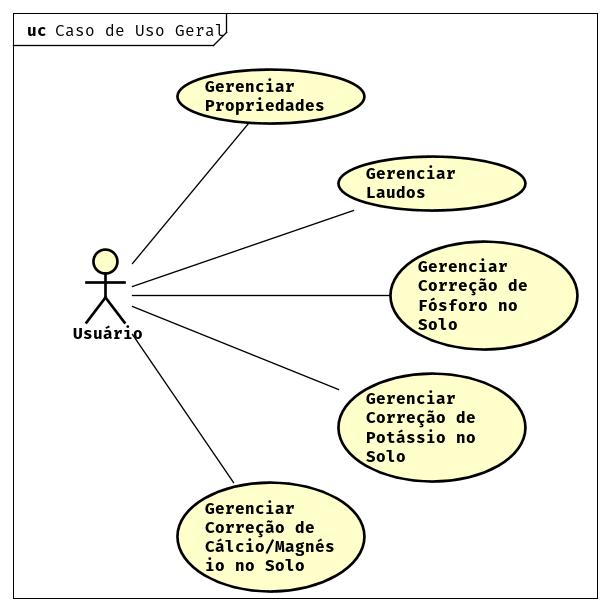
\includegraphics[width=13cm]{dados/figuras/casouso.jpg}
    \label{fig:diagramaCasoUso}
    \fonte{Autoria própria}
\end{figure}

Os casos de uso estão intimamente relacionados aos requisitos funcionais enumerados na \autoref{rf:tabela} e que serão comentados nas subseções abaixo.

\subsubsection{Caso de Uso - Gerenciar propriedades}
\label{sec:titSecCasoUsoPropriedades}

O Caso de Uso "Gerenciar propriedades" está relacionado ao requisito funcional RF001. Um propriedade representa uma área pertencente à um agricultor, como um sítio ou fazenda. Cada propriedade possui uma ou várias partições ou talhões, que será analisada, sendo assim, de suma importância para o funcionamento da aplicação. Como um produtor pode ter várias áreas analisadas em uma propriedades, faz-se necessário a criação de uma entidade no sistema.

\subsubsection{Caso de Uso - Gerenciar laudos}
\label{sec:titSecCasoUsoLaudos}

O caso de uso "Gerenciar laudos" referencia os RF02 a RF06. O laudo técnico do solo representa os indicadores de nutrientes do solo de um determinado talhão. Um talhão pode ser analisado diversas vezes. Por isso é importante que este laudo seja gerenciável como uma entidade na aplicação.

\subsubsection{Caso de Uso - Gerenciar correção de fósforo no solo}
\label{sec:titSecCasoUsoFosforo}

O caso de uso "Gerenciar correção de fósforo no solo" referencia os RF07 a RF09. As variáveis de correção do solo são: fonte de corretivo, eficiência, custo por tonelada. As fontes de corretivo possuem um valor padrão, que o usuário poderá editar no momento da realização do cálculo pois um determinado corretivo pode ser vendido com o mesmo nome mas ter propriedades diferentes. Por isso é necessário tornar gerenciável.

\subsubsection{Caso de Uso - Gerenciar correção de potássio no solo}
\label{sec:titSecCasoUsoPotassio}

O caso de uso "Gerenciar correção de potássio no solo" referencia os RF10 a RF12. Caso a saturação de bases fique além do ideal, é possível alterar o percentual desejado de potássio na CTC. Também deve ser possível o usuário alterar o valor em R\$/ton da fonte de potássio.

\subsubsection{Caso de Uso - Gerenciar correção do cálcio e magnésio no solo}
\label{sec:titSecCasoUsoCalcioMagnesio}

O caso de uso "Gerenciar correção do cálcio e magnésio no solo" referencia os RF13 a RF25. Caso a saturação de bases fique além do necessário, o usuário do sistema poderá corrigir o percentual de cálcio desejado na CTC. Além disso, também deve ser possível o usuário alterar o valor padrão do PRNT do corretivo, bem como o valor em R\$/ton.
\clearpage

\section{Diagrama de Classes}
\label{sec:titSecDiagClasse}

O Diagrama de Classes, segundo \cite{guedes2018uml}, define a estrutura das classes utilizadas pelo sistema, determinando os atributos e métodos que cada classe tem, além de estabelecer como as classes se relacionam e trocam informações entre si. A aplicação desse diagrama no sitema em questão pode ser vista na \autoref{fig:diagramaClasse}.

\begin{figure}[H]
    \centering
    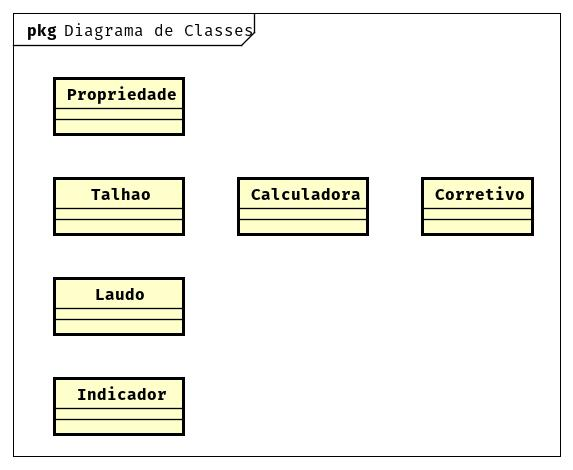
\includegraphics[width=13cm]{./dados/analise/diagramaclasse.jpg}
    \caption{Diagrama de Classes}
    \label{fig:diagramaClasse}
\end{figure}
\clearpage

\section{Projeto de Banco de Dados}
\label{sec:titSecBancoDados}

Segundo \cite{silberschatz2006sistema}, o objetivo do projeto de Banco de Dados é a construção de um conjunto de estruturas que permitam a representação de um dado de forma não redundante e que esse dado possa ser recuperado de forma simples. Este processo geralmente passa em diferentes níveis de abstração. Primeiramente, inicia-se com o entendimento do problema, para depois seguir por diferentes fases de modelagem, até chegar à implementação. Nesse processo, um modelo considerado padrão para a etapa inicial de modelagem é o entidade-relacionamento (ER) \cite{heuser2009projeto}.

\subsection{Diagrama de Entidade-Relacionamento}
\label{sec:titSecDiagER}

A modelagem entidade-relacionamento é a mais utilizada e difundida técnica de modelagem de dados. Nesta técnica, o modelo de dados é representado por meio de um modelo entidade-relacionamento (modelo ER). Comumente, o modelo ER é representado graficamente por meio de um diagrama entidade-relacionamento (DER) \cite{heuser2009projeto}.

A \autoref{fig:diagramaer} representa o DER do projetado neste documento.

\begin{figure}[H]
    \centering
    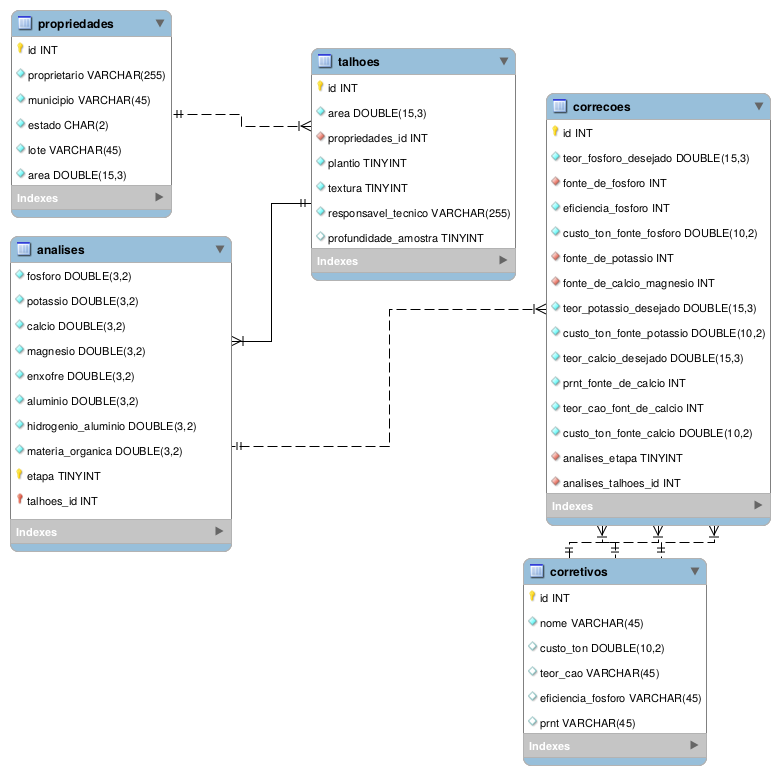
\includegraphics[width=13cm]{./dados/analise/diagramaer.png}
    \caption{Diagrama Entidade-Relacionamento}
    \label{fig:diagramaer}
\end{figure}

\subsection{Dicionário de Dados}
\label{sec:titSecDiagERDicionario}

\begin{landscape}
    \subsubsection{Tabela de Propriedades}
    \label{sec:titSubSecPropriedades}

    \begin{table}[H]
        \centering
        \caption[Tabela \textbf{propriedades}]{Na tabela propriedades ficarão armazenados os dados referentes à propriedade.
            \label{tab:tabela-er-propriedades}}
        \begin{tabular}{|p{4cm}|p{3cm}|p{2cm}|p{1cm}|p{2cm}|p{8cm}|}
            \hline
            Atributo     & Classe       & Domínio  & Bytes & Restrição & Descrição            \\\hline
            id           & Determinante & Numérico & 4     & PK, AI    &                      \\\hline
            proprietario & Simples      & Texto    & 255   & NN        & Nome do proprietário \\\hline
            municipio    & Simples      & Texto    & 255   & NN        & e.g. Dois Vizinhos   \\\hline
            estado       & Simples      & Texto    & 2     & NN        & e.g. PR              \\\hline
            lote         & Simples      & Texto    & 20    & NN        & e.g Q-103            \\\hline
            area         & Simples      & Numérico & 255   & NN        & Em metros quadrados  \\\hline
        \end{tabular}
    \end{table}

    \subsubsection{Tabela de Talhões}
    \label{sec:titSubSecTalhoes}

    \begin{table}[H]
        \centering
        \caption[Tabela \textbf{talhões}]{Na tabela talhões serão armazenados os dados referentes aos talhões da propriedade.
            \label{tab:tabela-er-talhoes}}
        \begin{tabular}{|p{4cm}|p{3cm}|p{2cm}|p{1cm}|p{2cm}|p{8cm}|}
            \hline
            Atributo              & Classe       & Domínio    & Bytes & Restrição & Descrição                        \\\hline
            id                    & Determinante & Numérico   & 4     & PK, AI    &                                  \\\hline
            area                  & Simples      & Numérico   & 10    & NN        & Em metros quadrados              \\\hline
            propriedades\_id      & Composto     & Numérico   & 255   & FK, NN    & Referência à tabela propriedades \\\hline
            plantio               & Simples      & Enumeravel & 1     & NN        & e.g. 1 (Plantio Direto)          \\\hline
            textura               & Simples      & Enumeravel & 1     & NN        & e.g. 2 (Textura Média)           \\\hline
            responsavel\_tecnico  & Simples      & Texto      & 255   & NN        & e.g. Pedro Cecere Filho          \\\hline
            profundidade\_amostra & Simples      & Numérico   & 255   &           & Em centímetros                   \\\hline
        \end{tabular}
    \end{table}

    \subsubsection{Tabela de Análises}
    \label{sec:titSubSecAnalises}

    \begin{table}[H]
        \centering
        \caption[Tabela \textbf{análises}]{Na tabela análises serão armazenados os dados do laudo técnico referente ao talhão.
            \label{tab:tabela-er-analises}}
        \begin{tabular}{|p{4cm}|p{3cm}|p{2cm}|p{1cm}|p{2cm}|p{8cm}|}
            \hline
            Atributo             & Classe       & Domínio  & Bytes & Restrição & Descrição                          \\\hline
            fosforo              & Simples      & Numérico & 4     & NN        & centimol de carga/decimetro cúbico \\\hline
            potassio             & Simples      & Numérico & 4     & NN        & centimol de carga/decimetro cúbico \\\hline
            calcio               & Simples      & Numérico & 4     & NN        & centimol de carga/decimetro cúbico \\\hline
            magnesio             & Simples      & Numérico & 4     & NN        & centimol de carga/decimetro cúbico \\\hline
            enxofre              & Simples      & Numérico & 4     & NN        & centimol de carga/decimetro cúbico \\\hline
            aluminio             & Simples      & Numérico & 4     & NN        & centimol de carga/decimetro cúbico \\\hline
            hidrogenio\_aluminio & Simples      & Numérico & 4     & NN        & centimol de carga/decimetro cúbico \\\hline
            materia\_organica    & Simples      & Numérico & 4     & NN        & centimol de carga/decimetro cúbico \\\hline
            etapa                & Determinante & Numérico & 4     & PK, AI    &                                    \\\hline
            talhoes\_id          & Composto     & Numérico & 4     & PK, FK    & Referência à tabela talhoes        \\\hline
        \end{tabular}
    \end{table}

    \subsubsection{Tabela de Correções}
    \label{sec:titSubSecAnalises}

    \begin{table}[H]
        \centering
        \caption[Tabela \textbf{Correções}]{Na tabela Correções serão armazenados os dados úteis para o cálculo do equilíbrio e correção do solo.
            \label{tab:tabela-er-correcoes}}
        \begin{tabular}{|p{4cm}|p{3cm}|p{2cm}|p{1cm}|p{2cm}|p{8cm}|}
            \hline
            Atributo                    & Classe       & Domínio  & Bytes & Restrição & Descrição                         \\\hline
            id                          & Determinante & Numérico & 4     & PK, AI    &                                   \\\hline
            teor\_fosforo\_desejado     & Simples      & Numérico & 1     & NN        & em percentual                     \\\hline
            fonte\_de\_fosforo          & Composto     & Numérico & 4     & NN        & em referência à tabela corretivos \\\hline
            eficiencia\_fosforo         & Simples      & Numérico & 1     & NN        & em percentual                     \\\hline
            custo\_ton\_fonte\_fosforo  & Simples      & Numérico & 8     & NN        & em R\$/tonelada                   \\\hline
            fonte\_de\_potassio         & Composto     & Numérico & 4     & NN        & em referência à tabela corretivos \\\hline
            fonte\_de\_calcio\_magnesio & Composto     & Numérico & 4     & NN        & em referência à tabela corretivos \\\hline
            teor\_potassio\_desejado    & Simples      & Numérico & 1     & NN        & em percentual                     \\\hline
            custo\_ton\_fonte\_potassio & Simples      & Numérico & 8     & NN        & em R\$/tonelada                   \\\hline
            teor\_calcio\_desejado      & Simples      & Numérico & 1     & NN        & em percentual                     \\\hline
            prnt\_fonte\_de\_calcio     & Simples      & Numérico & 1     & NN        & em percentual                     \\\hline
            teor\_cao\_font\_de\_calcio & Simples      & Numérico & 1     & NN        & em percentual                     \\\hline
            custo\_ton\_fonte\_calcio   & Simples      & Numérico & 8     & NN        & em R\$/tonelada                   \\\hline
            analises\_etapa             & Composto     & Numérico & 4     & FK        & Referência à tabela talhoes       \\\hline
            analises\_talhoes\_id       & Composto     & Numérico & 4     & FK        & Referência à tabela talhoes       \\\hline
        \end{tabular}
    \end{table}

    \subsubsection{Tabela de Correções}
    \label{sec:titSubSecAnalises}

    \begin{table}[H]
        \centering
        \caption[Tabela \textbf{Corretivos}]{Na tabela Corretivos serão armazenados os dados padrões acerca dos corretivos.
            \label{tab:tabela-er-correcoes}}
        \begin{tabular}{|p{4cm}|p{3cm}|p{2cm}|p{1cm}|p{2cm}|p{8cm}|}
            \hline
            Atributo            & Classe       & Domínio  & Bytes & Restrição & Descrição       \\\hline
            id                  & Determinante & Numérico & 4     & PK, AI    &                 \\\hline
            nome                & Simples      & Texto    & 255   & NN        & em percentual   \\\hline
            custo\_ton          & Simples      & Numérico & 8     &           & em R\$/tonelada \\\hline
            teor\_cao           & Simples      & Numérico & 1     &           & em percentual   \\\hline
            eficiencia\_fosforo & Simples      & Numérico & 1     &           & em percentual   \\\hline
            prnt                & Simples      & Numérico & 1     &           & em percentual   \\\hline
        \end{tabular}
    \end{table}

\end{landscape}
\clearpage

\subsection{Diagrama de Implantação}
\label{sec:titSecDiagDeploy}

O Diagrama de Implantação determina as necessidades de \textit{hardware} do sistema, as características físicas como servidores, estações, topologias e protocolos de comunicação \cite{guedes2018uml}, destacando todos as necessidades físicas no qual o sistema deverá ser executado. Também é mostrado como será a distribuição dos módulos do sistema nos momentos onde a aplicação estará sendo executada em diferentes servidores.

\begin{figure}[H]
    \centering
    \caption{Representação do Diagrama de Implantação}
    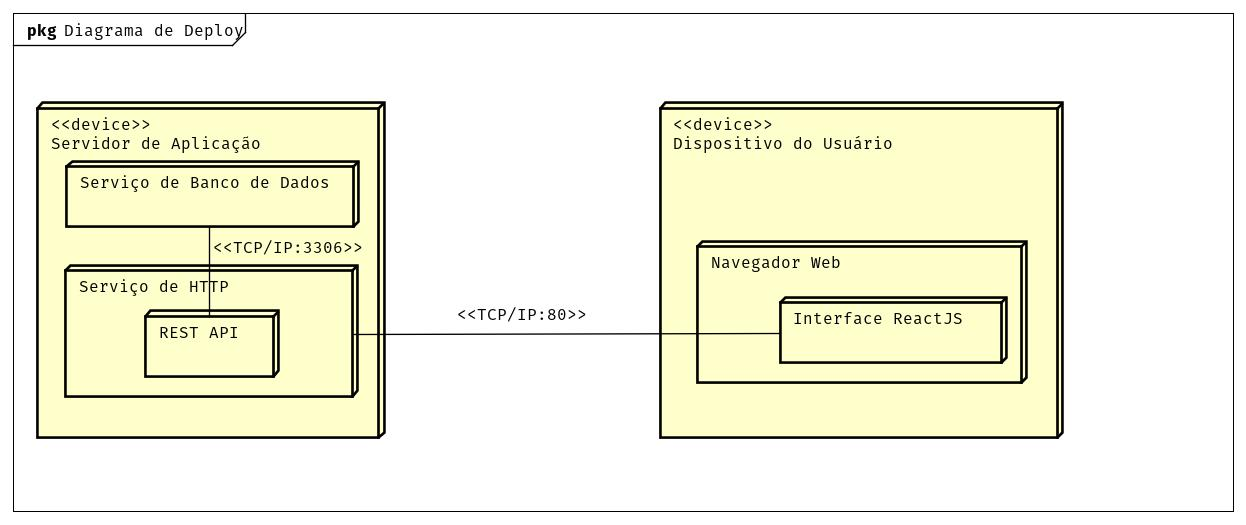
\includegraphics[width=13cm]{dados/figuras/diagramadeploy.jpg}
    \label{fig:diagramaDeploy}
    \fonte{Autoria própria}
\end{figure}

A \autoref{fig:diagramaDeploy} mostra a aplicação desse conceito no projeto. Nela é possível observar a distribuição do sistema em dois nós principais. O primeiro é o servidor de aplicação, que faz o encapsulamento do servidor Apache. Nesse mesmo servidor é possível observar a presença de um servidor MySQL, o qual será responsável por armazenar os dados do sistema e só receberá acessos locais.
O outro nó, representa o lado do cliente da aplicação, responsável pelas chamadas ao recursos contidos no servidor \textit{web} por meio de requisições Ajax, por meio do protocolo HTTP.

\clearpage

\section{PROTÓTIPOS DE TELA}
\label{sec:titSecPrototipos}

% Os protótipos de tela são uma versão inicial de um sistema. Eles são usados, dentre outras razões, para descobrir mais sobre um problema e suas possíveis soluções. O desenvolvimento rápido e iterativo do protótipo previne gastos desnecessários e custos controlados e os \textit{stakeholders} podem fazer usos pontuais de partes do sistema desde o início do desenvolvimento \citeonline{Sommerville10}.

% Além disso, os protótipos podem ajudar na antecipação de mudanças que podem ser requisitadas.
% Para o presente projeto foram desenvolvidas três interfaces para dois tamanhos diferentes de tela, simulando um dispositivo de tela maior (\textit{desktop}, \textit{tablet}) e outro para telas menores (\textit{smartphones}).

% O modelo de prototipação é ideal quando o cliente não tem os requisitos muito bem definidos, que é o caso do aplicativo estudado neste documento. Visto que os requisitos foram levantados com base em uma planilha, conforme explicado anteriormente na \autoref{sub:processo}.

Nas próximas subseções serão exibidos os protótipos de tela para três principais operações que o usuário poderá realizar no sistema, que são a tela que o usuário é enviado após fazer o \textit{login}, a tela para criação de um novo recurso no sistema e a tela de exibição de um recurso.

\subsection{Protótipos para tela inicial do sistema}
\label{sec:titSecPrototiposHome}

As Figuras \ref{fig:prototipo_home_desk} e \ref{fig:prototipo_home_mobile}, representam a visão da página inicial do sistema, que será exibida após o login do usuário. É possível observar que logo na parte superior, existirão quadros informativos sobre a quantidade de propriedades assistidas, quantidade de cidades atendidas e a área em hectares que foram tratadas (ou corrigidas). Logo abaixo serão exibidas as últimas correções realizadas pelo usuário.

\begin{figure}[H]
    \centering
    \caption{Página que será exibida após o login do usuário na visão de um dispositivo \textit{desktop}}
    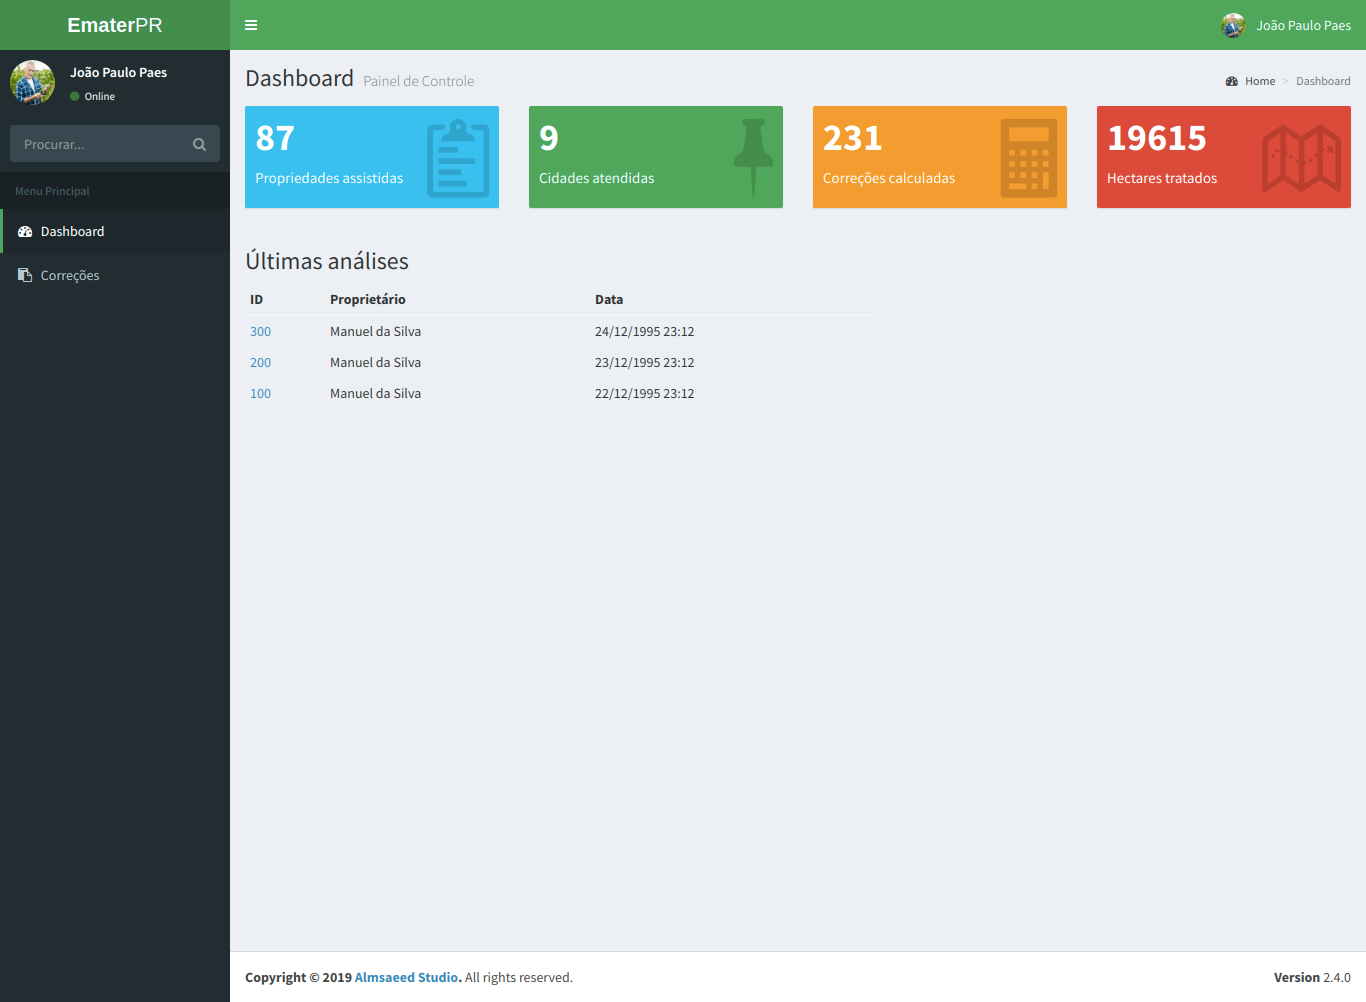
\includegraphics[width=13cm]{./dados/figuras/prototipos/home_desktop.png}
    \label{fig:prototipo_home_desk}
    \fonte{Autoria própria}
\end{figure}

\begin{figure}[H]
    \centering
    \caption{Página que será exibida após o login do usuário na visão de um dispositivo \textit{mobile}}
    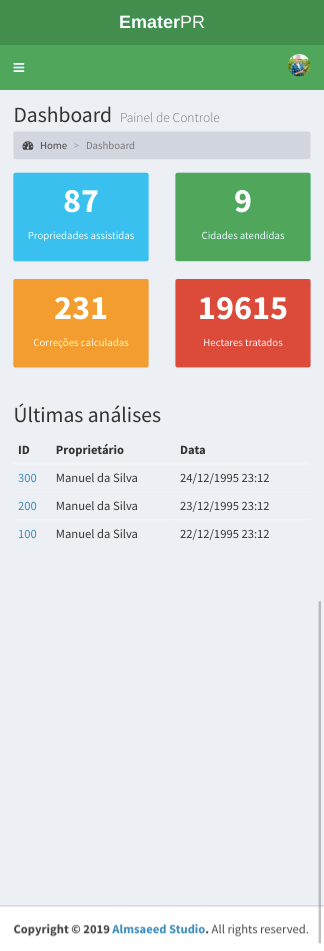
\includegraphics[width=6cm]{./dados/figuras/prototipos/home_mobile.png}
    \label{fig:prototipo_home_mobile}
    \fonte{Autoria própria}
\end{figure}

\subsection{Protótipos para tela de cadastro de informação}
\label{sec:titSecPrototiposCreate}

A tela de cadastro de informações foi pensada para ser intuitiva e reativa como a planilha. Como é um formulário grande, será divido em \textit{steps} que serão exibidos na parte superior do formulário, tendo a descrição do que deve ser feito naquele \textit{step} logo abaixo. Já o formulário propriamente dito terá uma interface reativa, que lembra a planilha.

No exemplo mostrado nas Figuras \ref{fig:prototipo_create_desk} e \ref{fig:prototipo_create_mobile}, é possível observar que caso o valor de um campo esteja no intervalo ideal, este deverá ter a sua \textit{label} e o contorno destacados em verde. Enquanto se o valor estiver fora do intervalo, em âmbar. 

\begin{figure}[H]
    \centering
    \caption{Criação de recurso na visão de um dispositivo \textit{desktop}}
    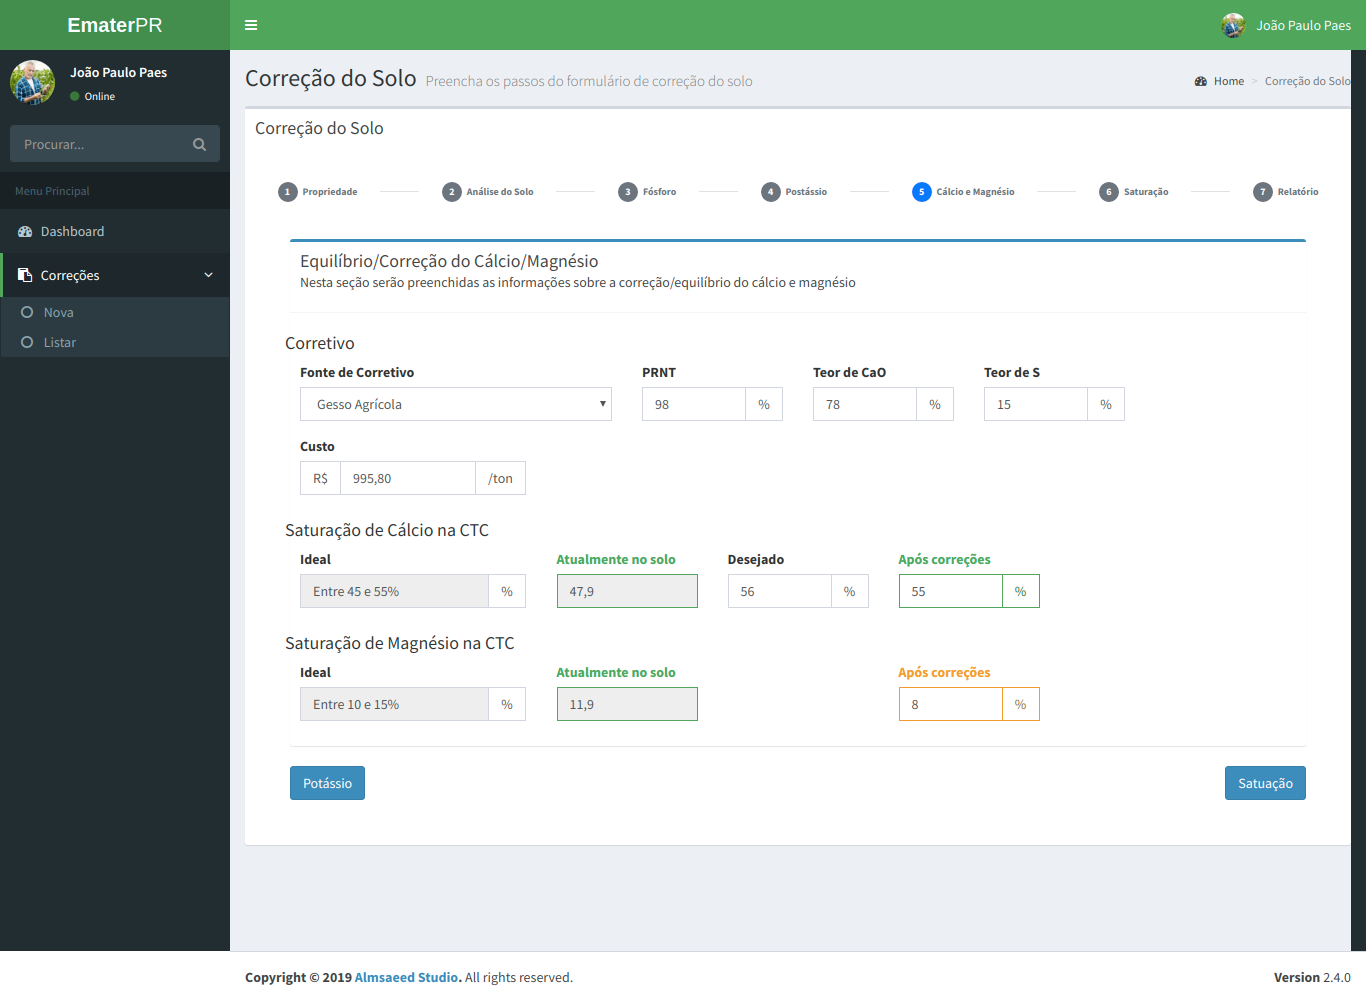
\includegraphics[width=13cm]{./dados/figuras/prototipos/create_desktop.png}
    \label{fig:prototipo_create_desk}
    \fonte{Autoria própria}
\end{figure}

\begin{figure}[H]
    \centering
    \caption{Criação de recurso na visão de um dispositivo \textit{mobile}}
    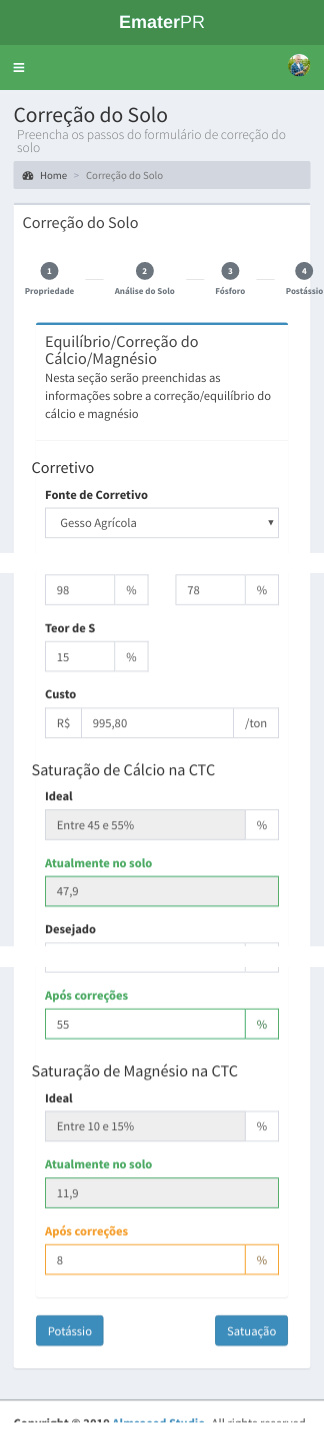
\includegraphics[width=6cm]{./dados/figuras/prototipos/create_mobile.png}
    \label{fig:prototipo_create_mobile}
    \fonte{Autoria própria}
\end{figure}


\subsection{Protótipos para tela de exibição de informação}
\label{sec:titSecPrototiposShow}

A tela de exibição da informação também seguirá o modelo de \textit{steps}. Ela deverá ser dividia em 3 colunas para representar os três estados da correção do solo: naquele momento, desejado e após as correções. É possível notar que os textos deverão estar coloridos de acordo com o caso no qual se encaixa. Acima do valor, amarelo. Abaixo do valor, vermelho. No intervalo, verde.

\begin{figure}[H]
    \centering
    \caption{Visualização de recurso na visão de um dispositivo \textit{desktop}}
    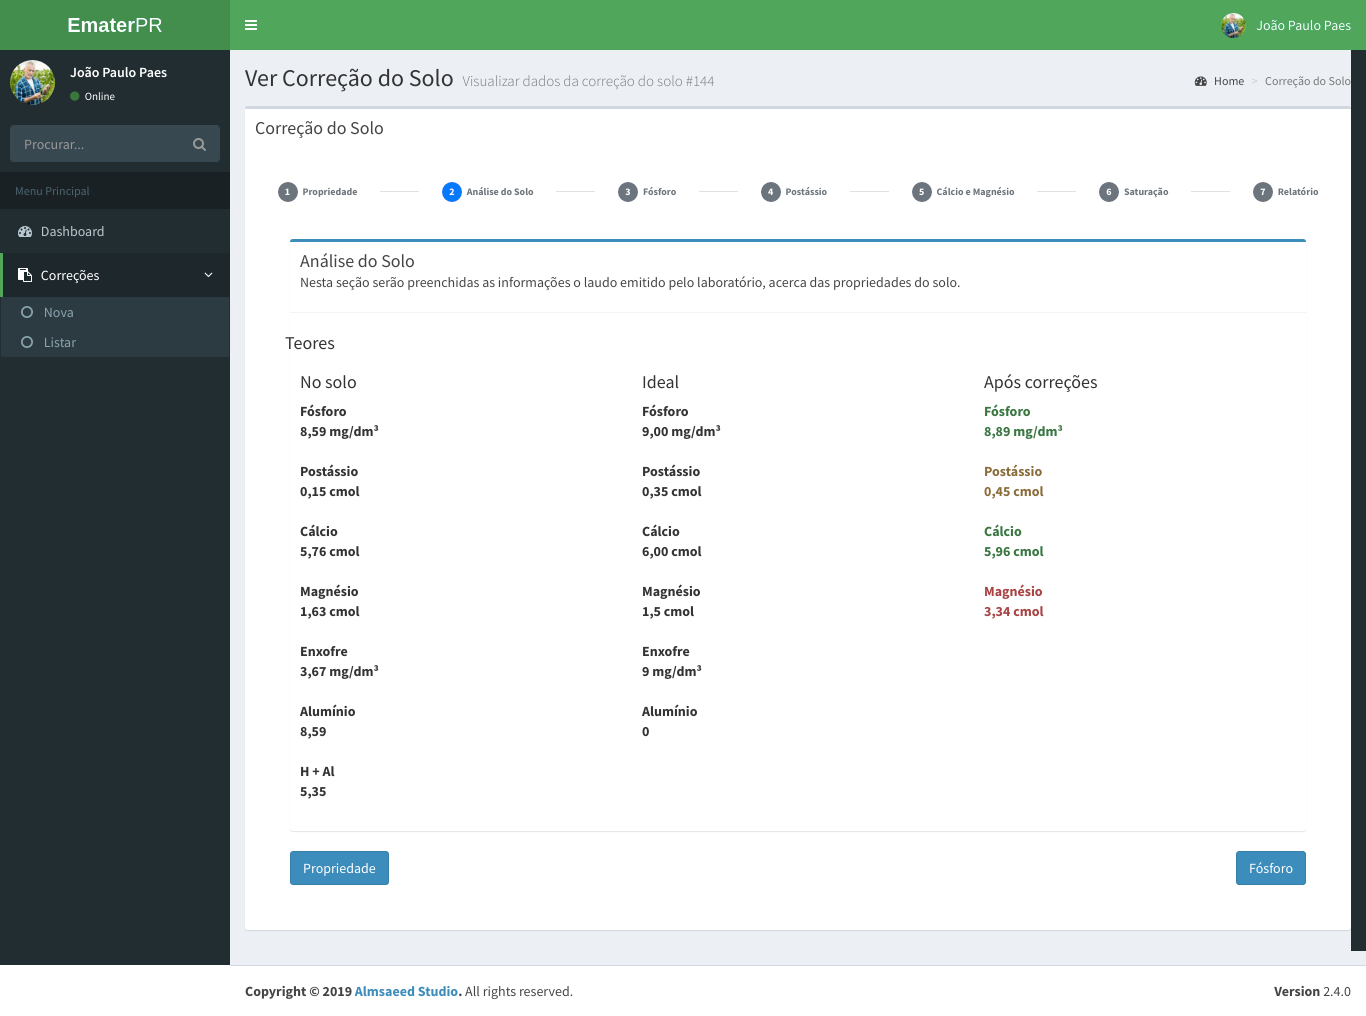
\includegraphics[width=13cm]{./dados/figuras/prototipos/show_desktop.png}
    \label{fig:prototipo_show_desk}
    \fonte{Autoria própria}
\end{figure}

\begin{figure}[H]
    \centering
    \caption{Visualização de recurso na visão de um dispositivo \textit{mobile}}
    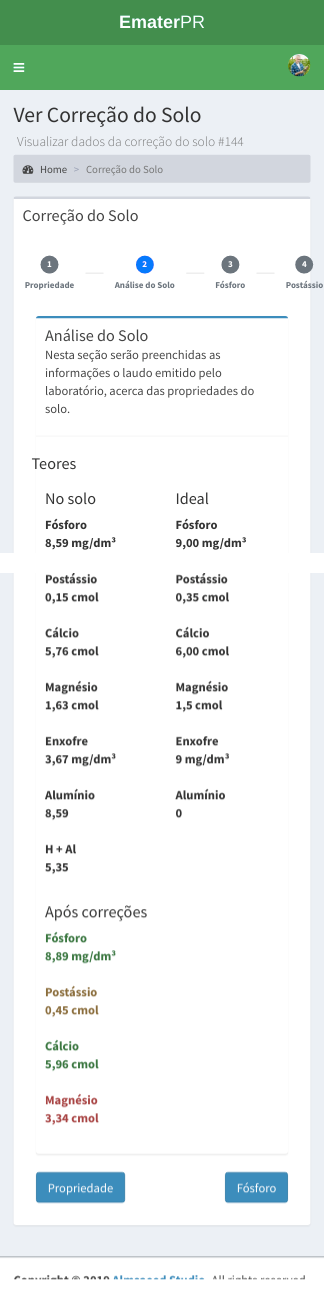
\includegraphics[width=6cm]{./dados/figuras/prototipos/show_mobile.png}
    \label{fig:prototipo_show_mobile}
    \fonte{Autoria própria}
\end{figure}
\clearpage                   % Análise
% CONCLUSÃO--------------------------------------------------------------------

\chapter{CONCLUSÃO}
\label{chap:conclusao}

Parte final do texto, na qual se apresentam as conclusões do trabalho acadêmico. É importante fazer uma análise crítica do trabalho, destacando os principais resultados e as contribuições do trabalho para a área de pesquisa.

\section{TRABALHOS FUTUROS}
\label{sec:trabalhosFuturos}

Também deve indicar, se possível e/ou conveniente, como o trabalho pode ser estendido ou aprimorado.

\section{CONSIDERAÇÕES FINAIS}
\label{sec:consideracoesFinais}

Encerramento do trabalho acadêmico.
                 			   % Conclusão

\postextual
% INSERE ELEMENTOS PÓS-TEXTUAIS
% REFERÊNCIAS------------------------------------------------------------------

% Carrega o arquivo "base-referencias.bib" e extrai automaticamente as referências citadas

\bibliography{./base-referencias}
\bibliographystyle{abntex2-alf} % Define o estilo ABNT para formatar a lista de referências
% OBSERVAÇÕES------------------------------------------------------------------
% Este arquivo não precisa ser alterado.
           			   % Referências
%% APÊNDICES--------------------------------------------------------------------

\begin{apendicesenv}
\partapendices

% Primeiro apêndice------------------------------------------------------------
\chapter{Nome do apêndice} % Edite para alterar o título deste apêndice
\label{chap:apendiceA}

Lembre-se que a diferença entre apêndice e anexo diz respeito à autoria do texto e/ou material ali colocado.

Caso o material ou texto suplementar ou complementar seja de sua autoria, então ele deverá ser colocado como um apêndice. Porém, caso a autoria seja de terceiros, então o material ou texto deverá ser colocado como anexo.

Caso seja conveniente, podem ser criados outros apêndices para o seu trabalho acadêmico. Basta recortar e colar este trecho neste mesmo documento. Lembre-se de alterar o "label"{} do apêndice.

Não é aconselhável colocar tudo que é complementar em um único apêndice. Organize os apêndices de modo que, em cada um deles, haja um único tipo de conteúdo. Isso facilita a leitura e compreensão para o leitor do trabalho.

% Novo apêndice----------------------------------------------------------------
\chapter{Nome do outro apêndice}
\label{chap:apendiceB}

conteúdo do novo apêndice

\end{apendicesenv}
             			   % Apêndices
% ANEXO------------------------------------------------------------------------

\begin{anexosenv}
\partanexos

% Primeiro anexo---------------------------------------------------------------
\chapter{Nome do anexo}     % edite para alterar o título deste anexo
\label{chap:anexoA}

Lembre-se que a diferença entre apêndice e anexo diz respeito à autoria do texto e/ou material ali colocado.

Caso o material ou texto suplementar ou complementar seja de sua autoria, então ele deverá ser colocado como um apêndice. Porém, caso a autoria seja de terceiros, então o material ou texto deverá ser colocado como anexo.

Caso seja conveniente, podem ser criados outros anexos para o seu trabalho acadêmico. Basta recortar e colar este trecho neste mesmo documento. Lembre-se de alterar o "label"{} do anexo.

Organize seus anexos de modo a que, em cada um deles, haja um único tipo de conteúdo. Isso facilita a leitura e compreensão para o leitor do trabalho. É para ele que você escreve.

% Novo anexo-------------------------------------------------------------------
\chapter{Nome do outro anexo}
\label{chap:anexoB}

conteúdo do outro anexo

\end{anexosenv}
               			   % Anexos

\end{document}
